%% Experimental validation 
\frame{
\begin{tikzpicture}[remember picture,overlay]
\fill[blue1]
(current page.north west) rectangle ([xshift=0.57\textwidth,yshift=0.28\textheight]current page.west|-{pic cs:end});
\end{tikzpicture}

\begin{textblock}{0.53}(0.02,0.03)
	\textcolor{white}{
	\Large Experimental validation of X-DFA: \\
	A suspension of sedimenting particles}
\end{textblock}

\begin{textblock}{0.57}(0.02,0.18)
\centering
\only<1>{
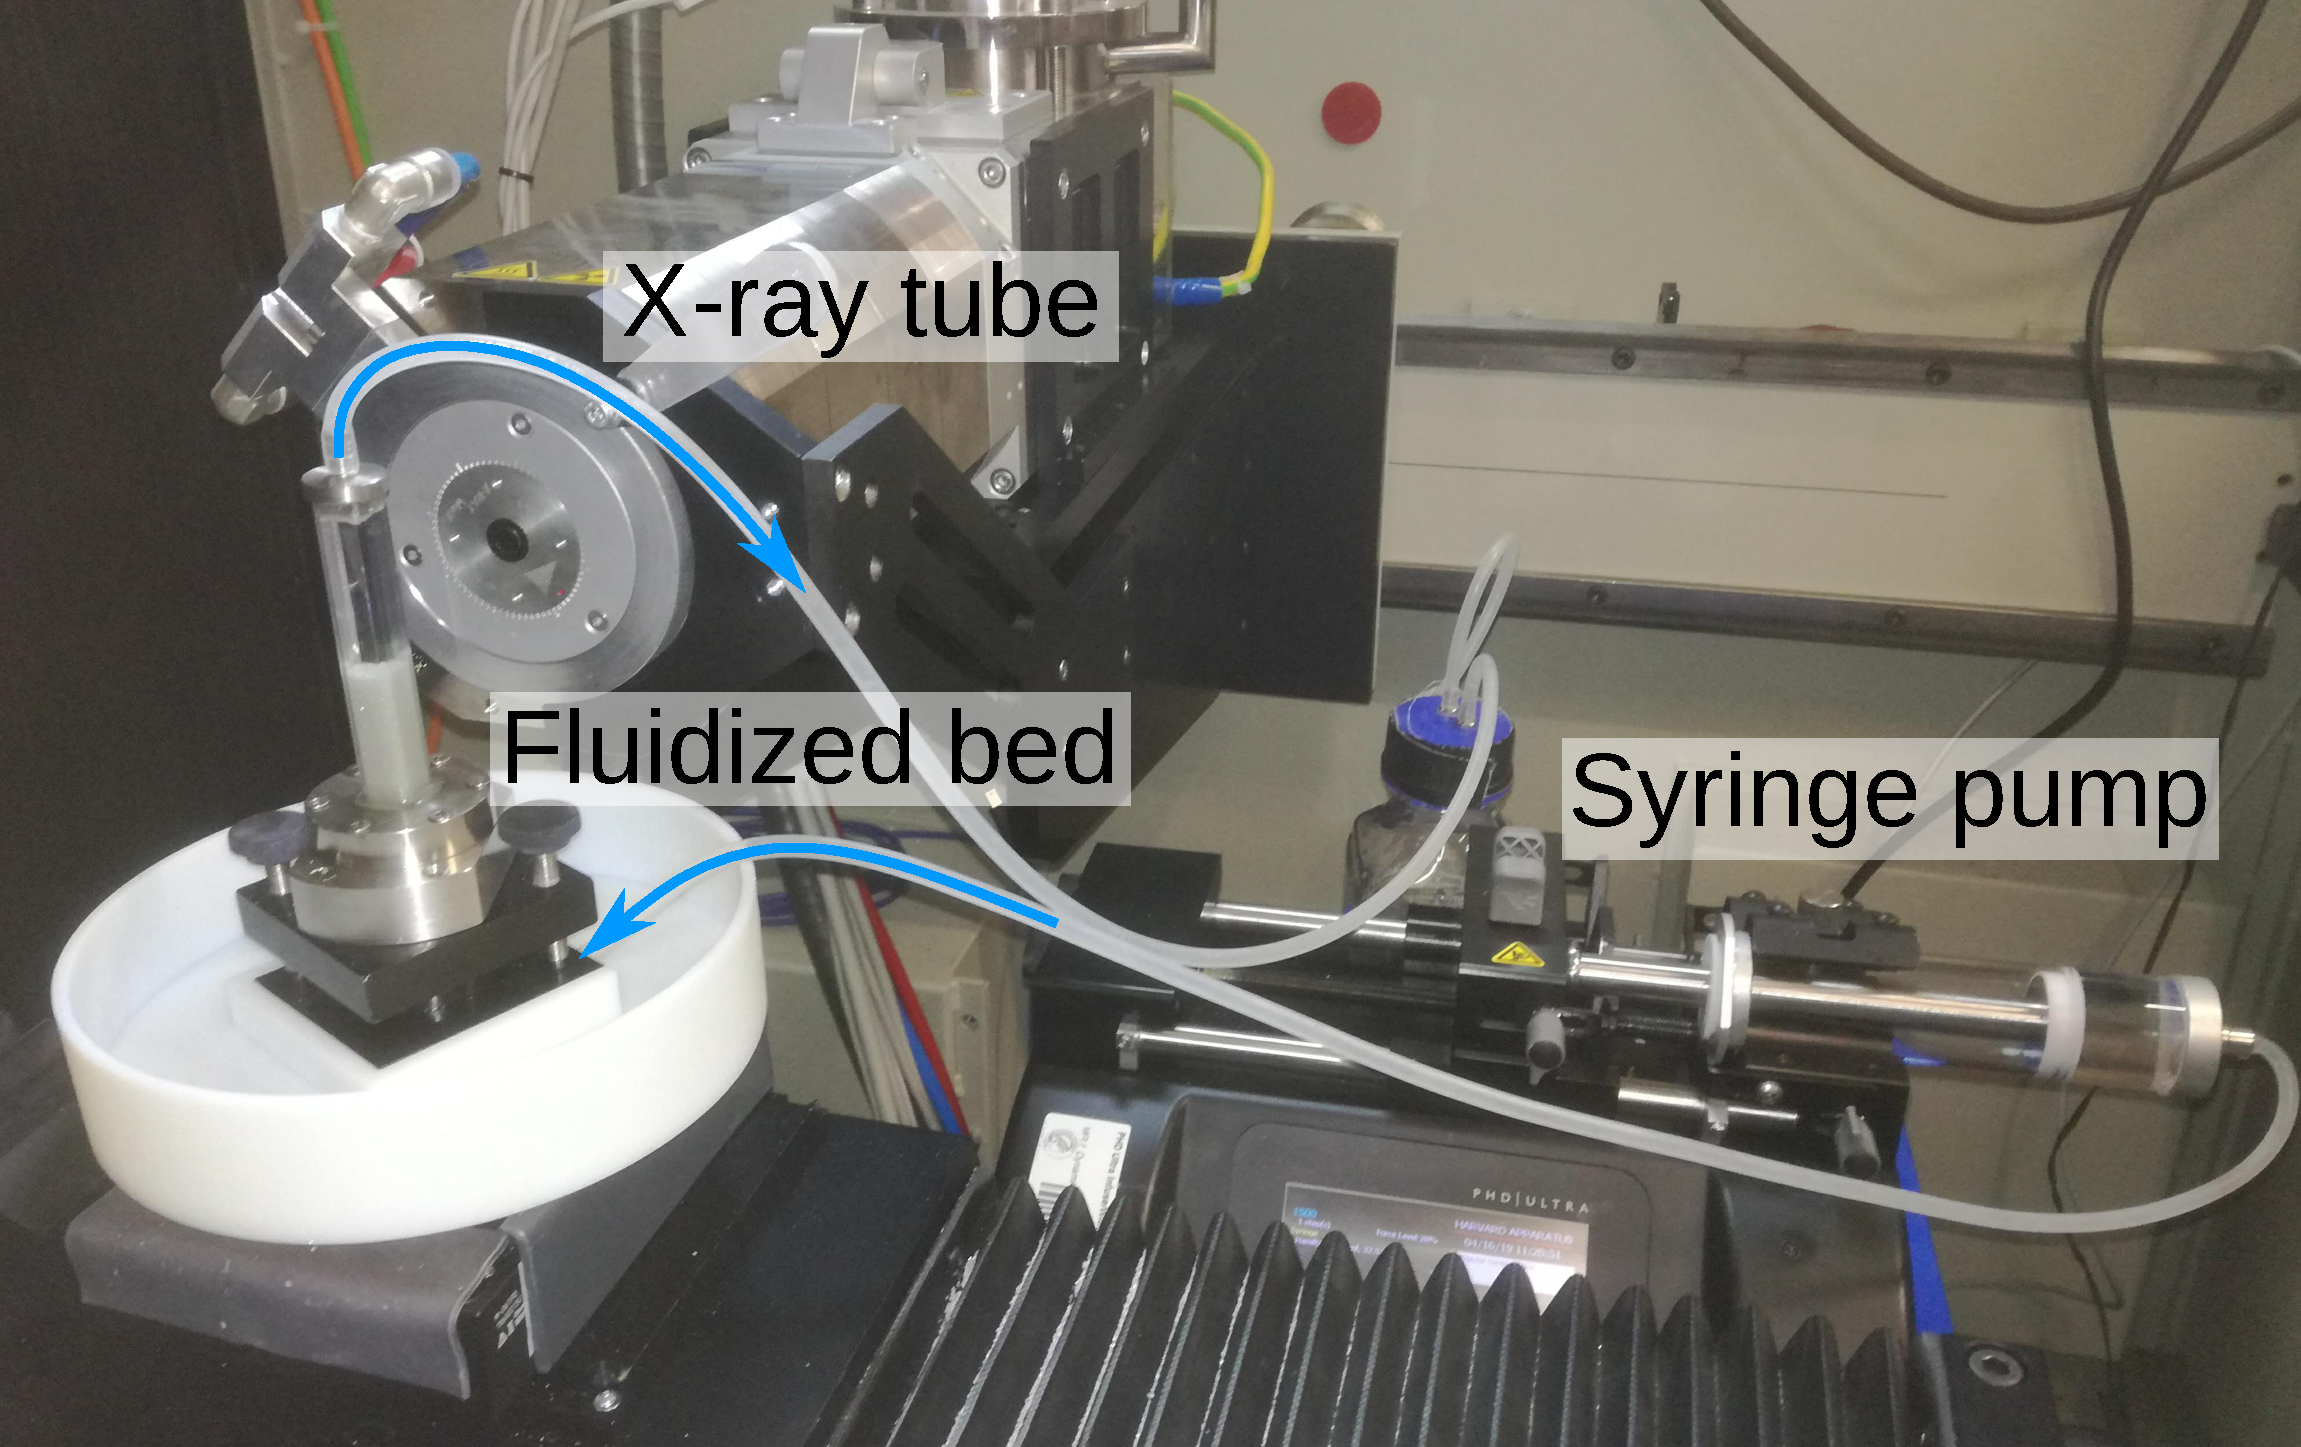
\includegraphics[width=\textwidth]{Sources/sedimenting_bed/Photo_fluidized_bed.pdf}
}
\visible<2->{
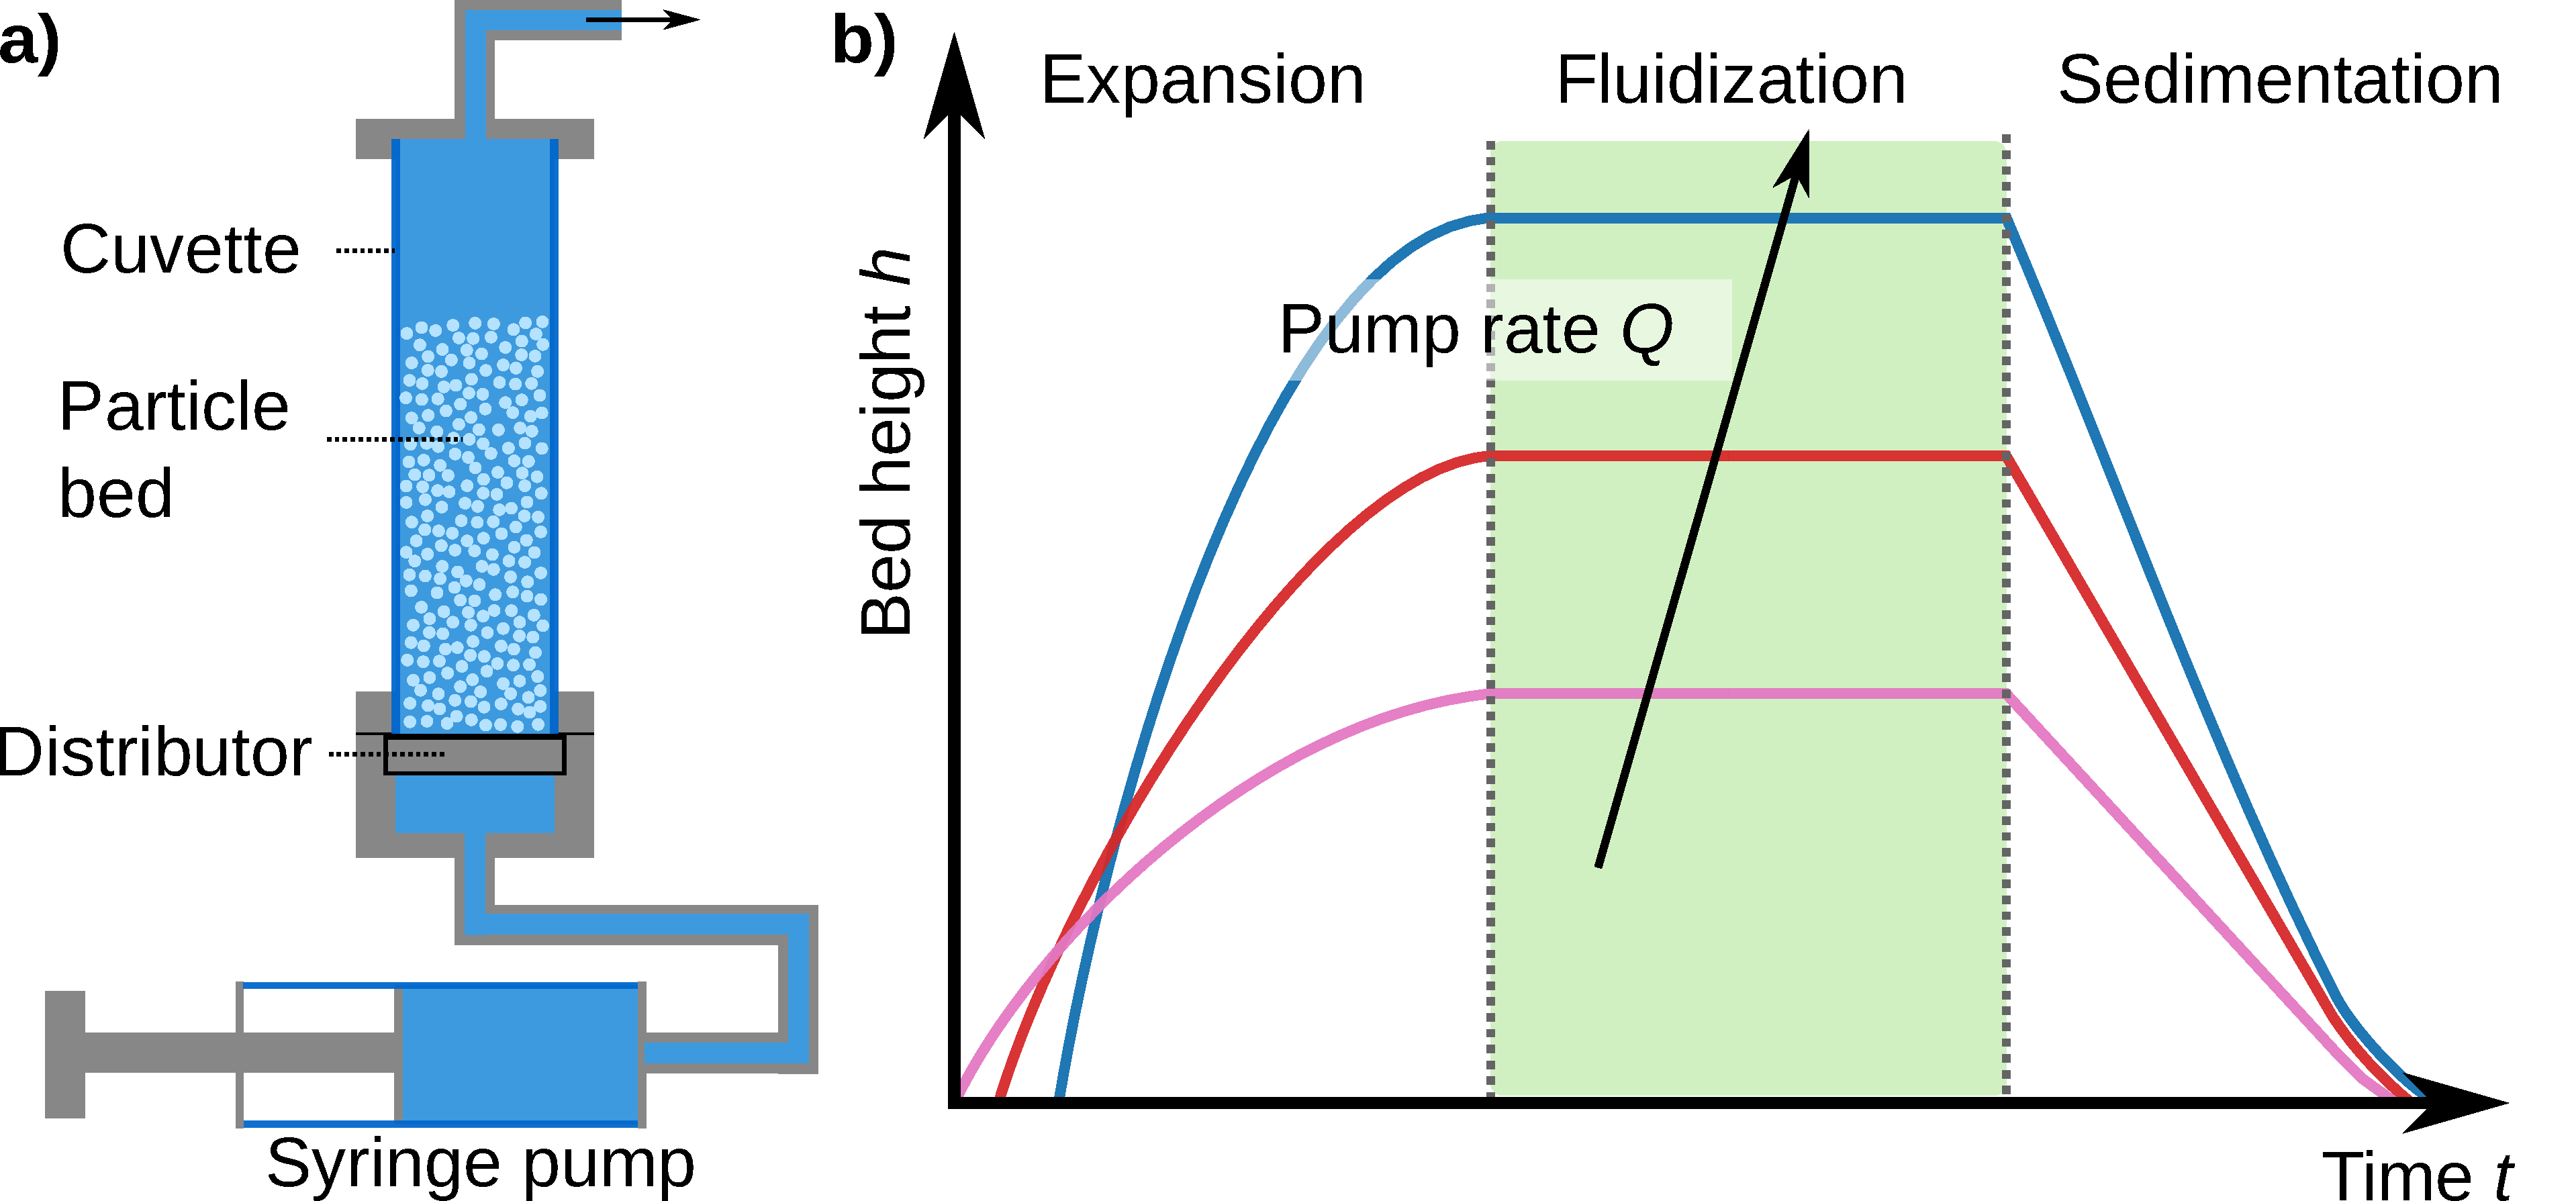
\includegraphics[width=\textwidth]{Sources/sedimenting_bed/setup-fluidized_bed_fluidized.pdf}}
\end{textblock}	

\begin{textblock}{0.28}(0.66,0.02)	
	\visible<2->{
	\centering
	X-ray radiography\\[0.1cm]
	\movie[width =\textwidth, poster, loop]
	{\includegraphics[width=\textwidth]{Sources/sedimenting_bed/Radiogram_plane.png}}
	{videos/full_fluidization1.avi}}
\end{textblock}

\begin{textblock}{0.38}(0.59,0.5)	
\visible<2->{
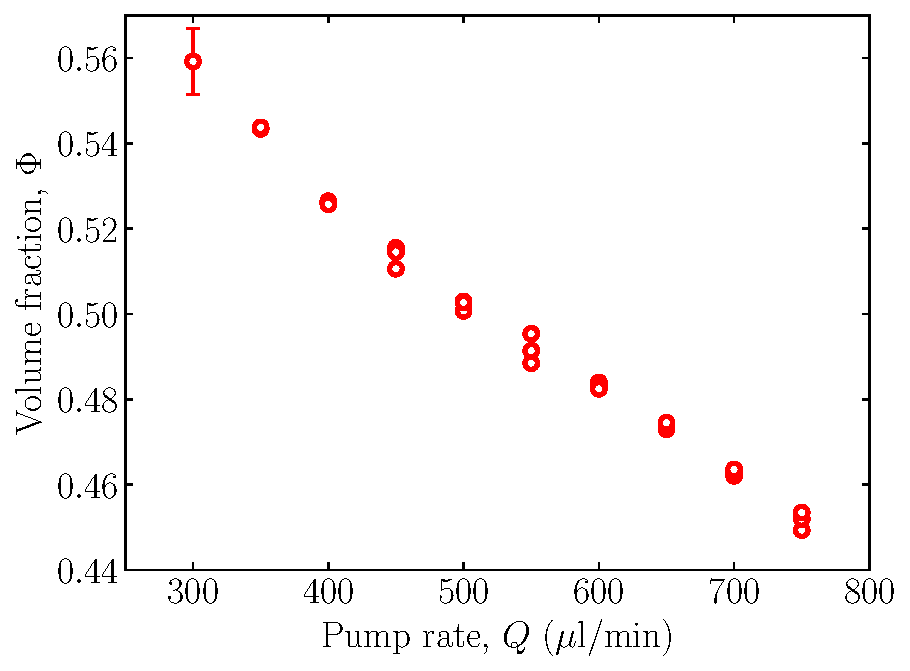
\includegraphics[width=\textwidth]{Sources/sedimenting_bed/Phi_vs_pump_rate.pdf}}
\end{textblock}

\begin{textblock}{0.35}(0.67,0.82)	
	\visible<2->{
		\colorbox{lightblue}{
			$0.45 <  \Phi < 0.56$}}
\end{textblock}

\begin{textblock}{0.15}(0.22,0.75)
	\only<3>{
	\textcolor{red}{No reliable reference velocity!}
	}
\end{textblock}

\begin{textblock}{0.17}(0.34,0.64)
	\only<3>{
	\fbox{\parbox{\textwidth}{
			\movie[width =\textwidth, poster, loop]
			{
\includegraphics[width=\textwidth]{Sources/X-DFA/cropped_80kV_340uA_38ms_0000.png}}
			{videos/fluidized_3500mul_per_min.avi}}}
		}
\end{textblock}
}



\begin{frame}[noframenumbering]
\begin{tikzpicture}[remember picture,overlay]
\fill[blue1]
(current page.north west) rectangle ([xshift=0.57\textwidth,yshift=0.28\textheight]current page.west|-{pic cs:end});
\end{tikzpicture}

\begin{textblock}{0.53}(0.02,0.03)
	\textcolor{white}{
		\Large Experimental validation of X-DFA: \\
		A suspension of sedimenting particles}
\end{textblock}

	
\begin{textblock}{0.57}(0.02,0.18)
	\centering
	\visible<1->{
	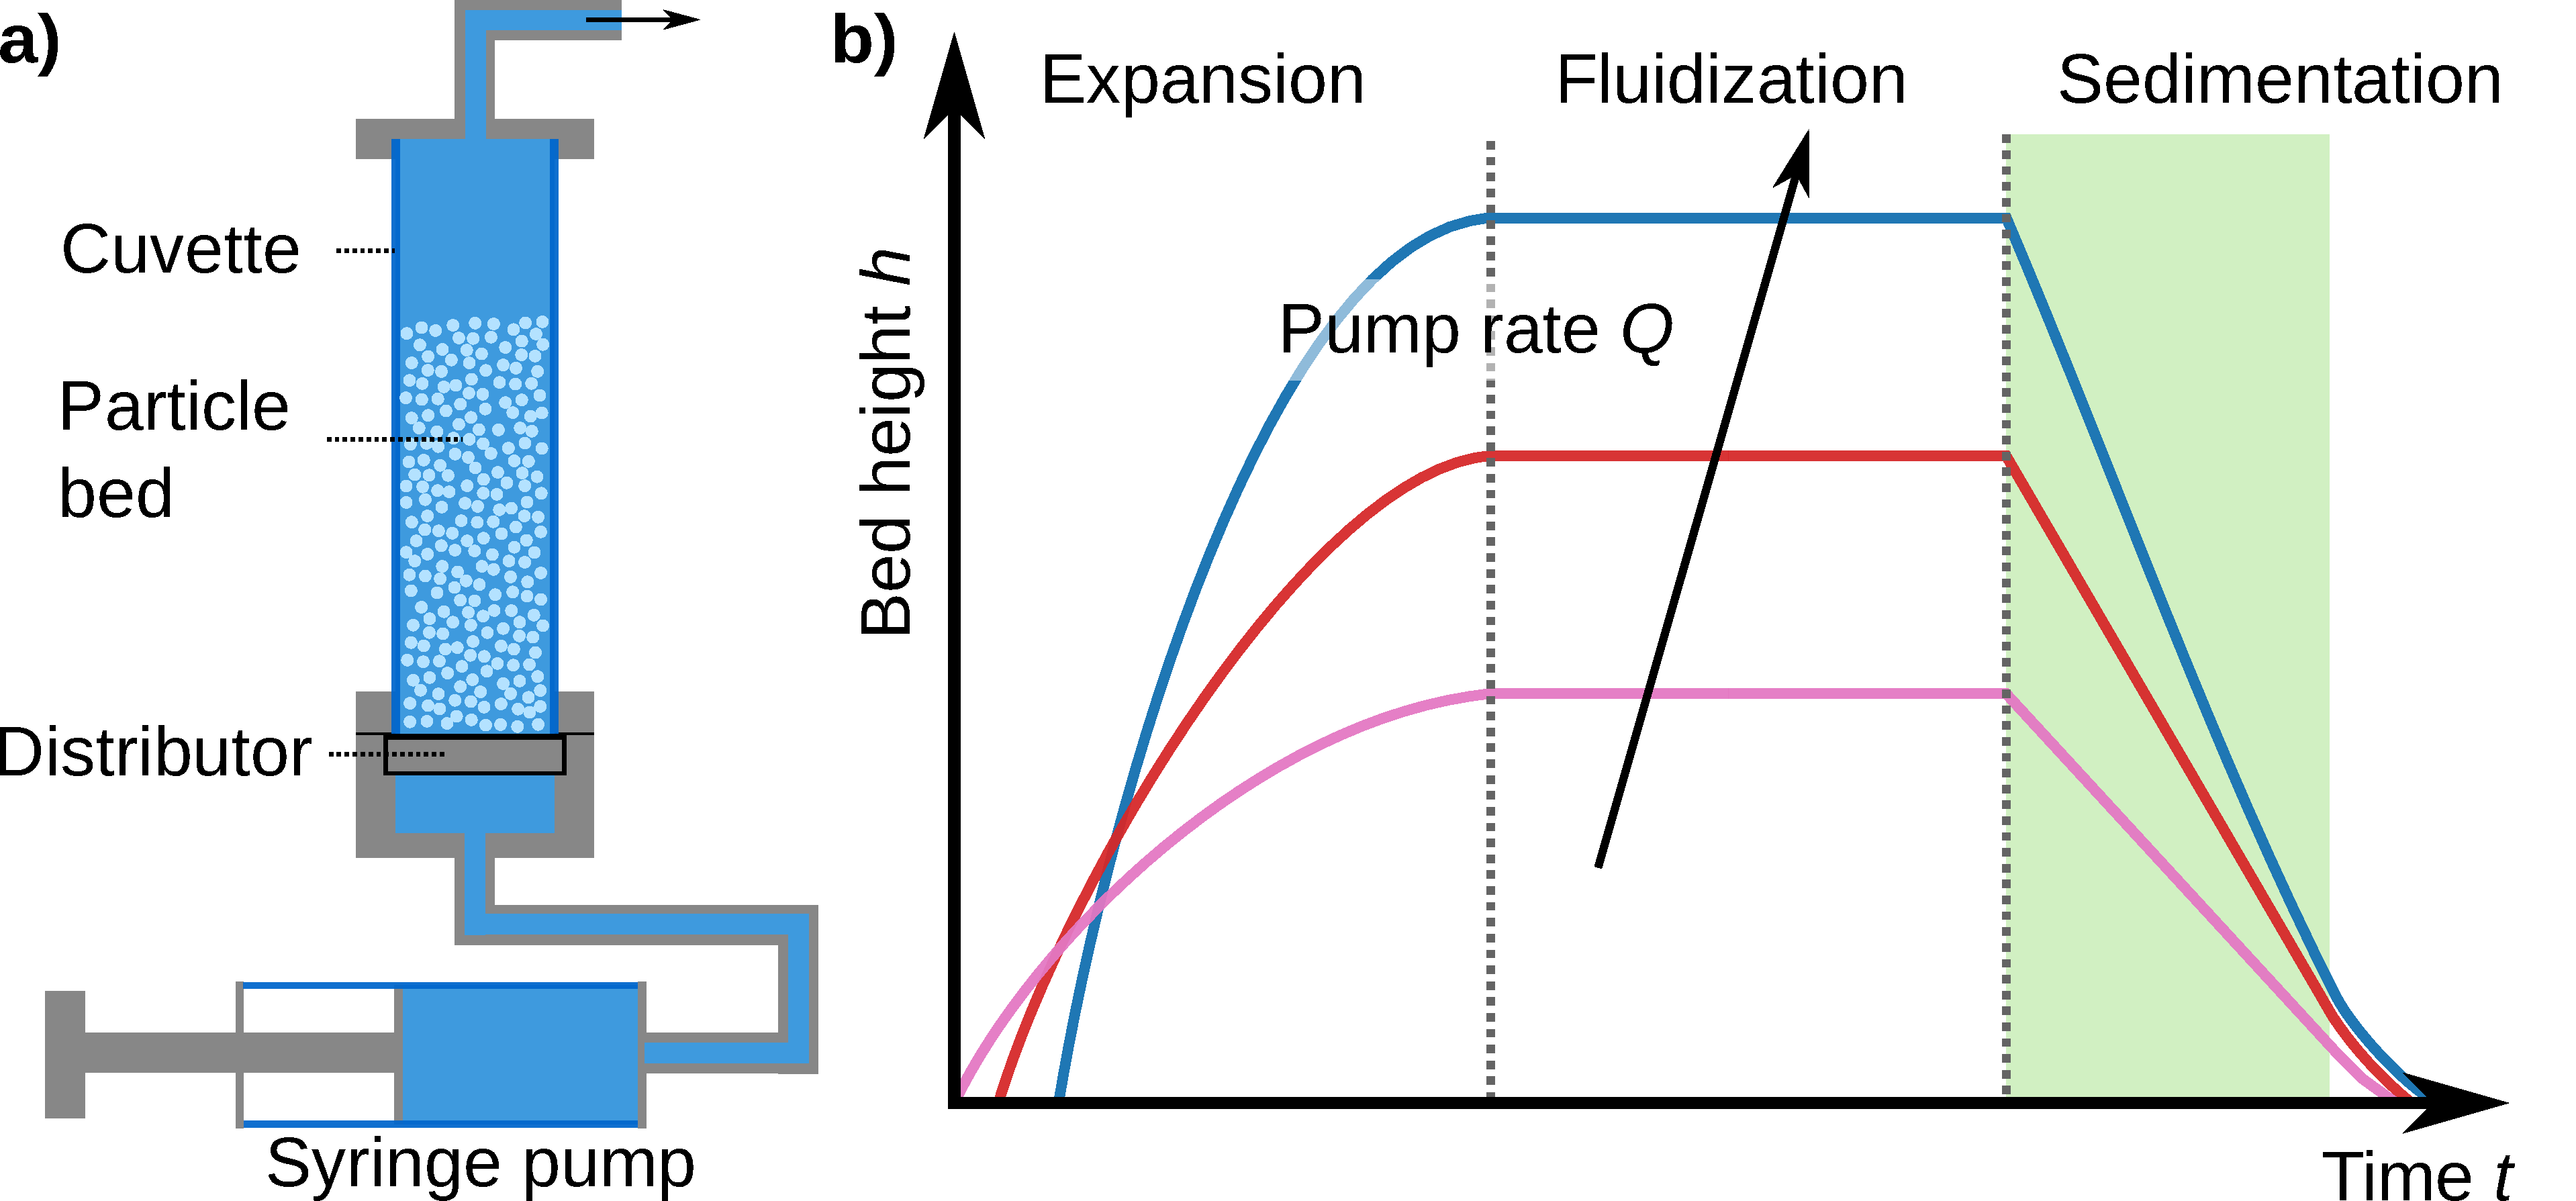
\includegraphics[width=\textwidth]{Sources/sedimenting_bed/setup-fluidized_bed.pdf}}
\end{textblock}	


\begin{textblock}{0.3}(0.66,0.05)
	\centering
	X-ray radiography\\[0.1cm]
	\only<1>{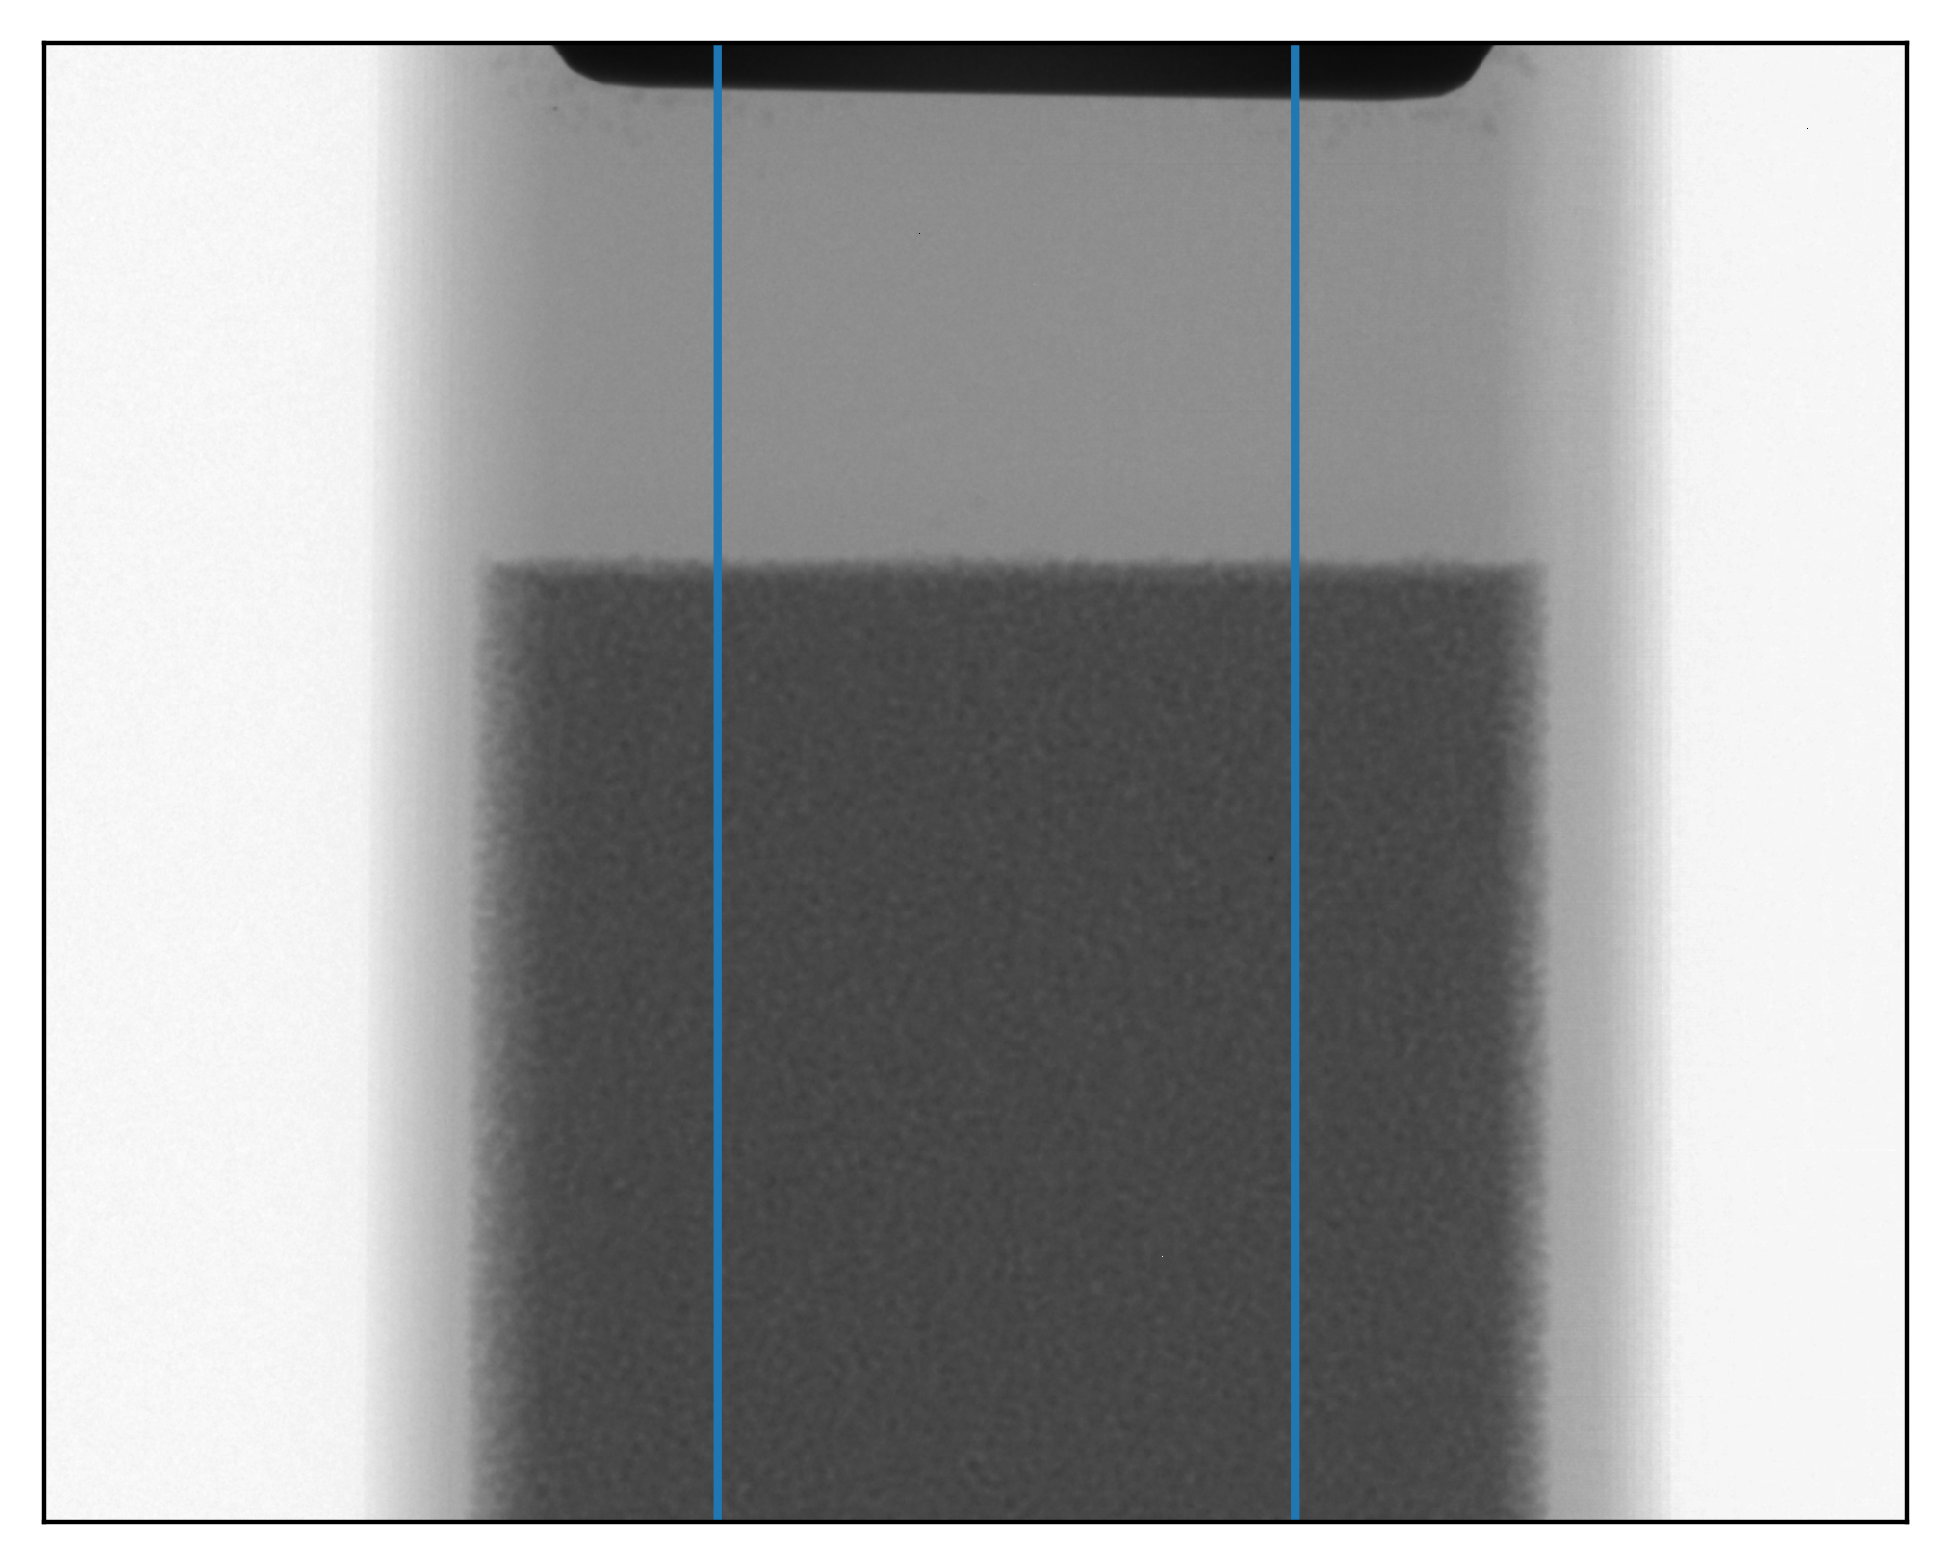
\includegraphics[width=\textwidth]{Sources/sedimenting_bed/ROI_marked_img_nr1.png}}
	\visible<2->{
	\fbox{\parbox{0.65\textwidth}{
	\movie[width = 0.65\textwidth, poster]
	{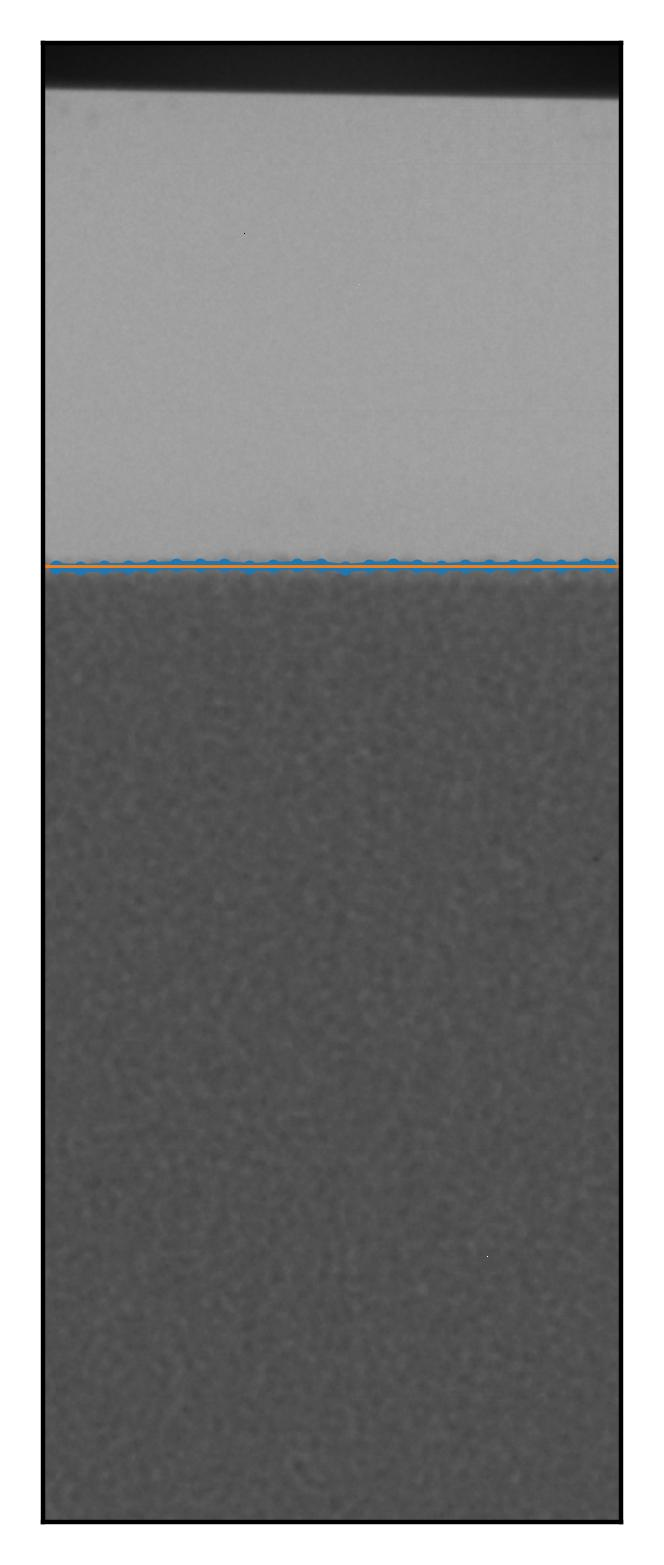
\includegraphics[width=.65\textwidth]{Sources/sedimenting_bed/tracked_edge0.png}}
	{videos/tracked_edge.avi}}}}
\end{textblock}

\begin{textblock}{0.17}(0.28,0.64)
	\visible<2->{
		\fbox{\parbox{\textwidth}{
		\movie[width =\textwidth, poster, loop]
		{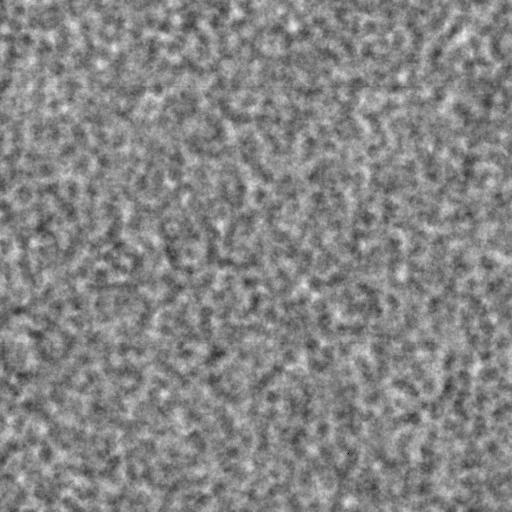
\includegraphics[width=\textwidth]{Sources/sedimenting_bed/sedimentationROI.png}}
		{videos/02_750ul_per_min_original.avi}}}
	}
\end{textblock}

\begin{textblock}{0.25}(0.45,0.75)
\visible<2->{
\centering
\textcolor{blue1}{
Comparison of \\
$\langle v \rangle_\text{xdfa}$ and $\langle v \rangle_\text{front}$}
}
\end{textblock}
\end{frame}

%%%%%%%%%%%%%%%%%% Sedimenting suspension: Richardson Zaki
\frame{	
	\begin{tikzpicture}[remember picture,overlay]
	\fill[blue1]
	(current page.north west) rectangle ([xshift=0.6\paperwidth,yshift=0.33\paperheight]current page.west|-{pic cs:end});
	\end{tikzpicture}
	
	\begin{textblock}{0.8}(0.02,0.03)
		\textcolor{white}{
			\Large Liquid fluidized bed: Richardson-Zaki law}
	\end{textblock}	
	
	\begin{textblock}{0.6}(0.02,0.2)
		\centering
		\only<1>{
		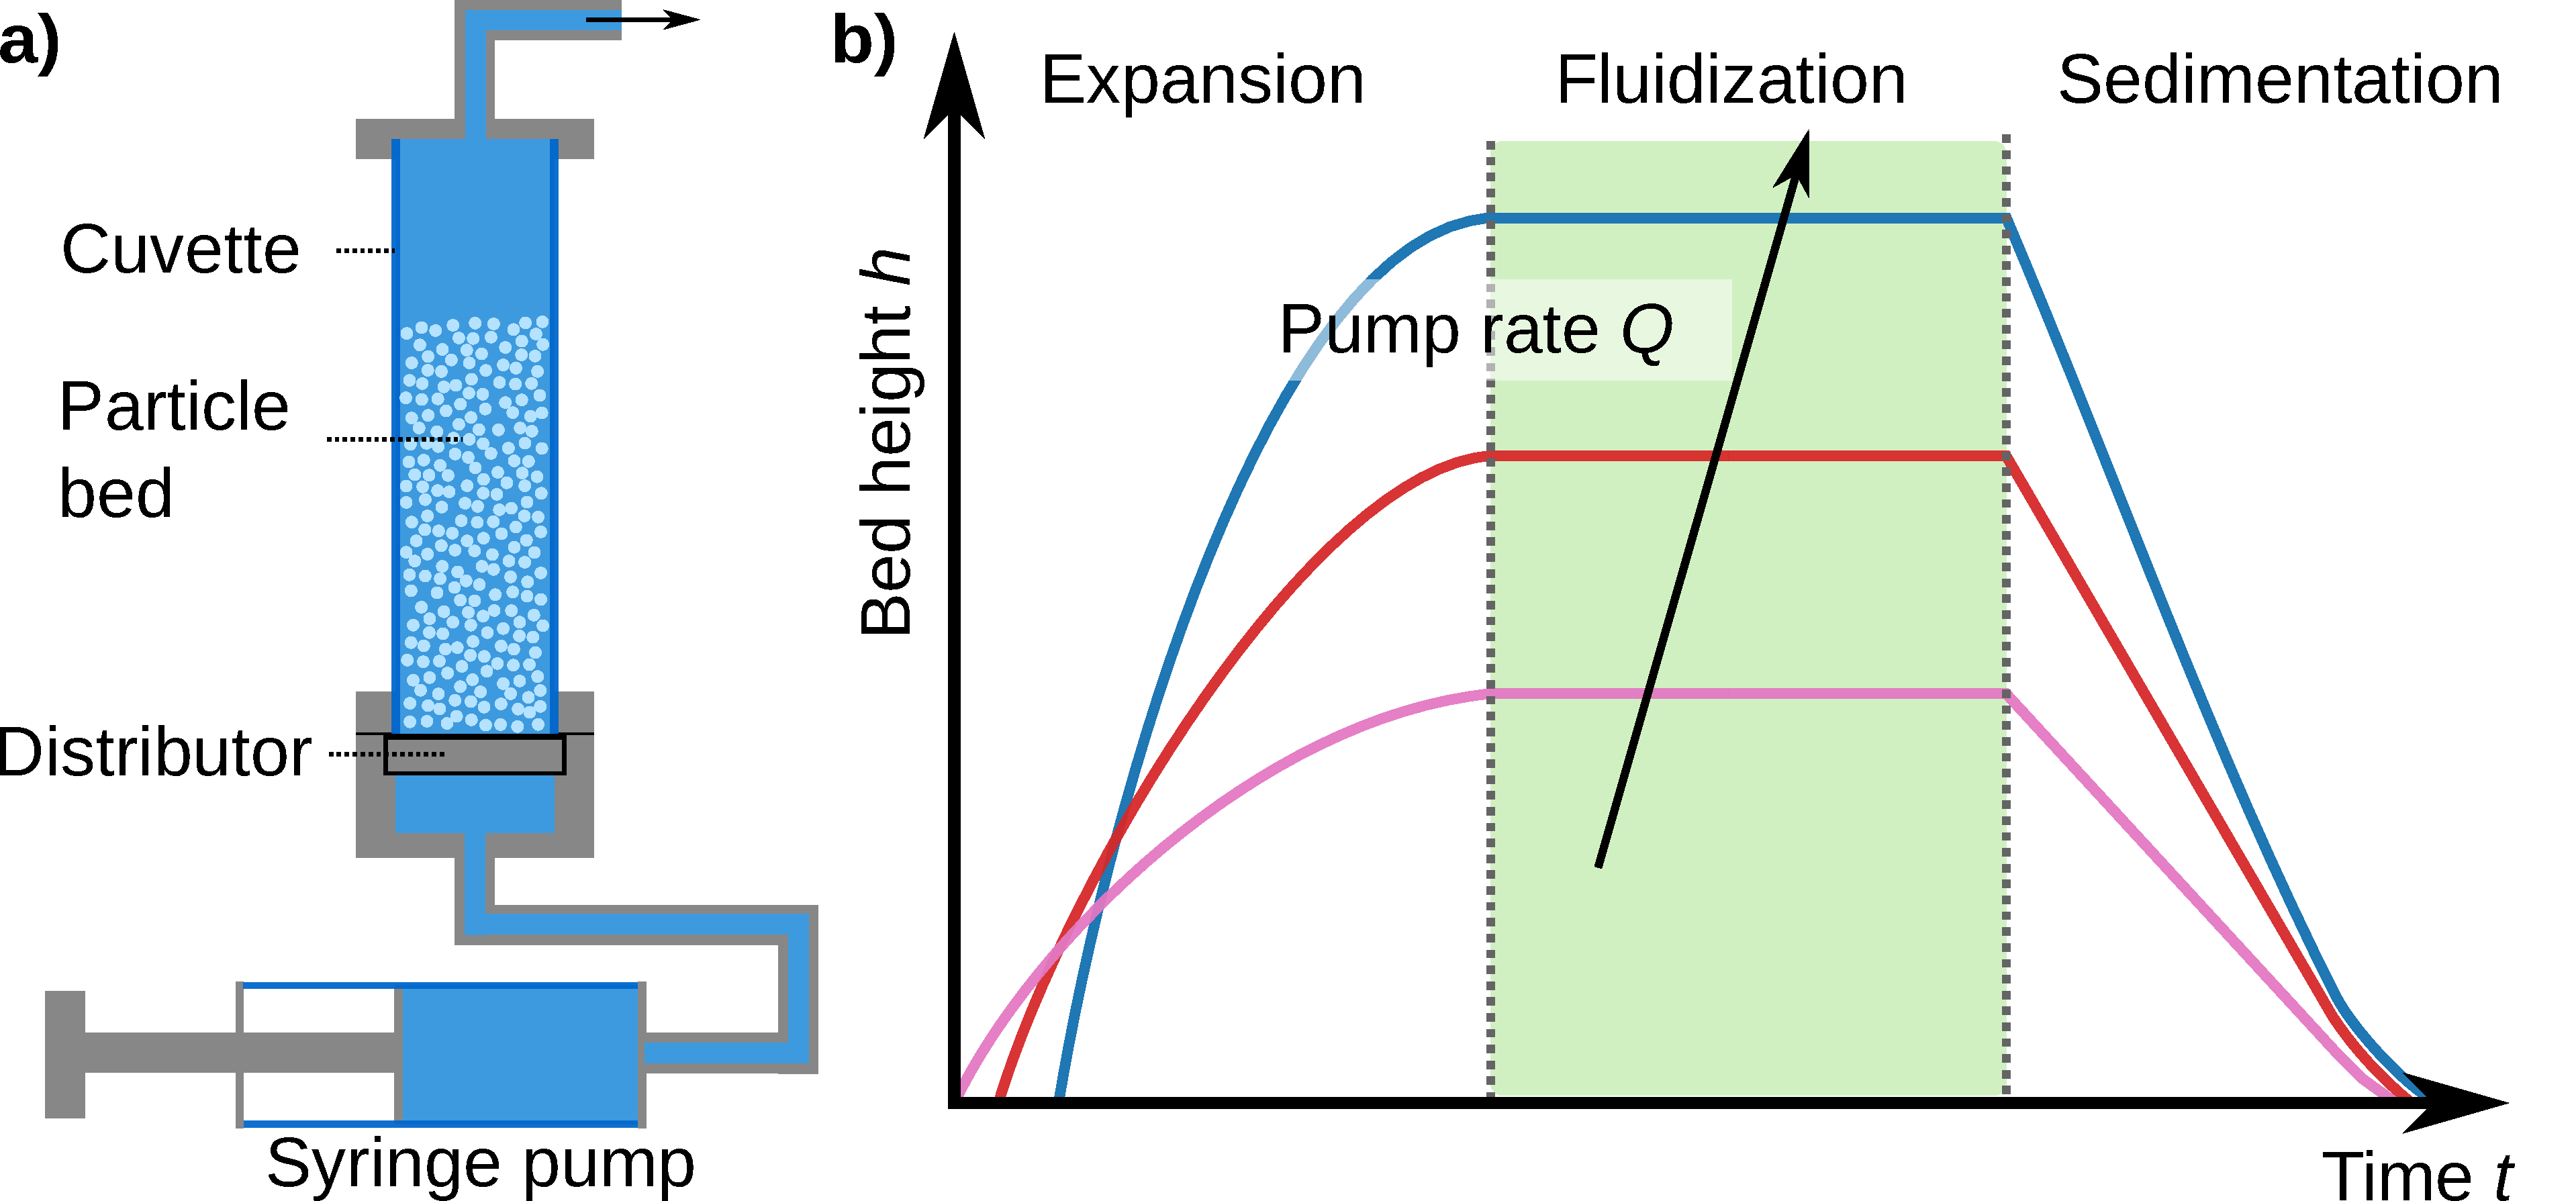
\includegraphics[width=\textwidth]
		{Sources/sedimenting_bed/setup-fluidized_bed_fluidized.pdf}}
		\visible<2->{
		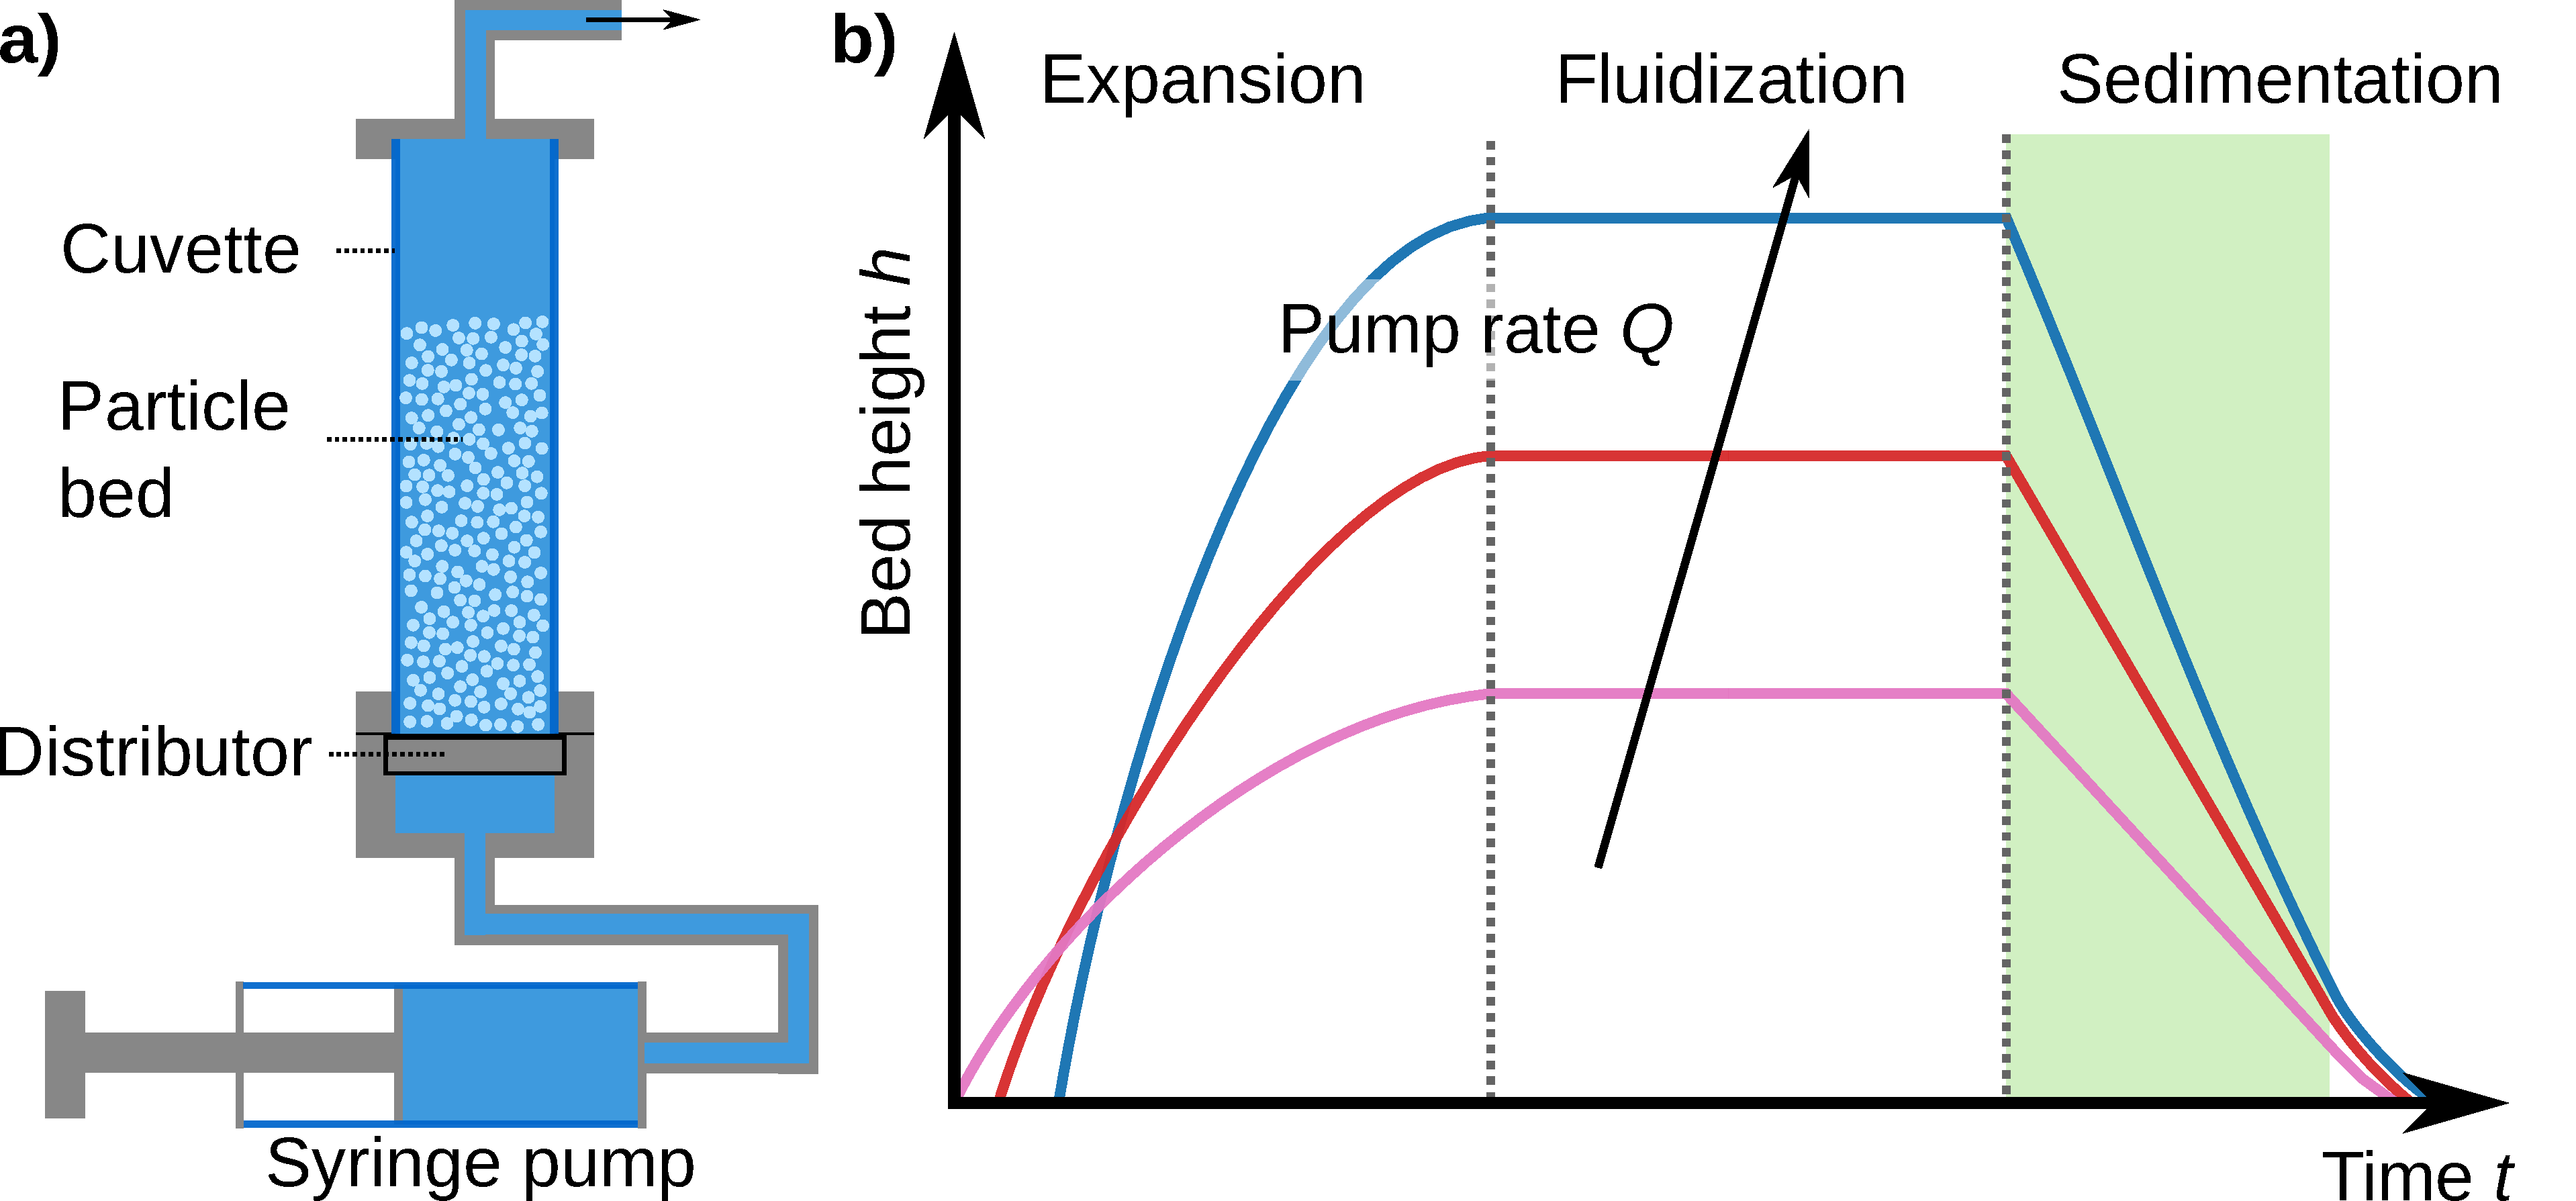
\includegraphics[width=\textwidth]{Sources/sedimenting_bed/setup-fluidized_bed.pdf}}
	\end{textblock}	
	
	\begin{textblock}{0.45}(0.6,0.05)
		\centering
		Gravitation \quad Buoyancy \quad Drag
		$F_\text{G} = F_\text{B} + F_\text{D}$	\\
		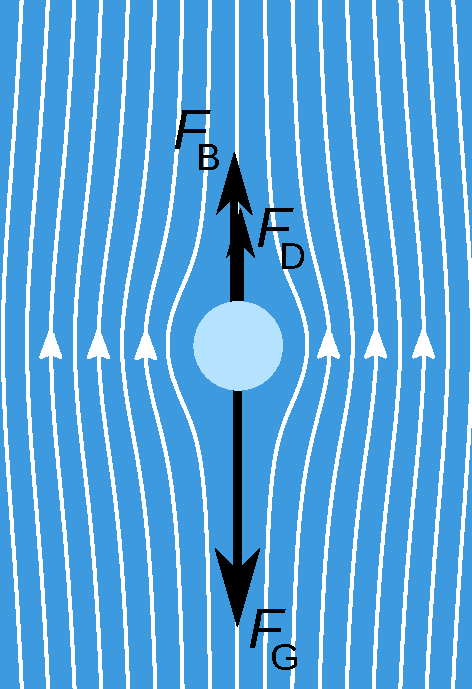
\includegraphics[width=0.3\textwidth]{Sources/sedimenting_bed/Drag_one.pdf}
	\end{textblock}
	
	\begin{textblock}{0.35}(0.62,0.5)
		\visible<2->{
		\centering
		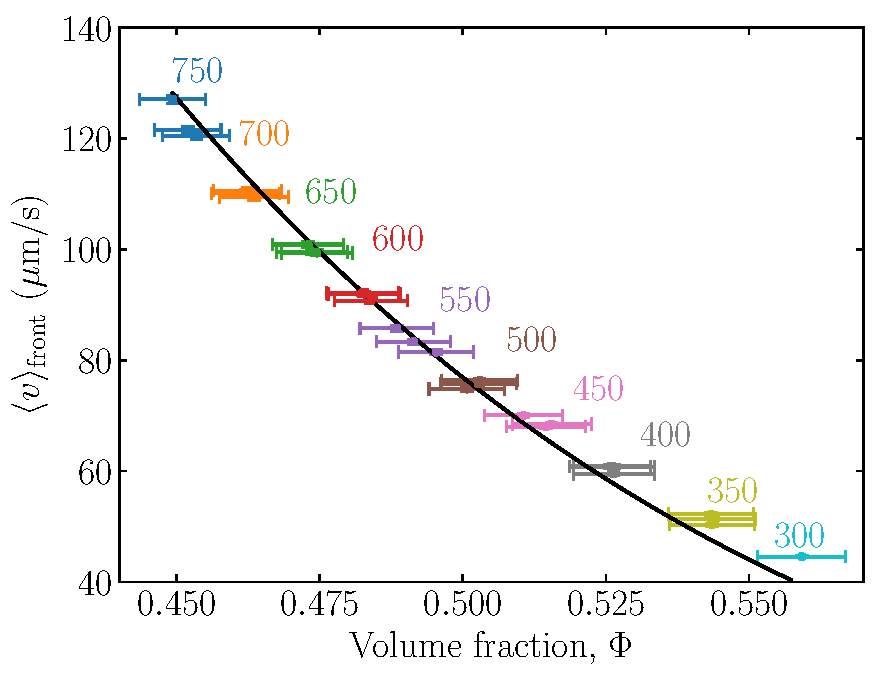
\includegraphics[width=\textwidth]
		{Sources/sedimenting_bed/Sed_vel_vs_Phi_fit_Richardson_Zaki.pdf}}
	\end{textblock}

	\begin{textblock}{0.2}(0.4,0.75)
	\only<1>{
		\[\frac{\langle v \rangle_\text{fluid}}{v_\text{Stokes}} = (1-\Phi)^n \]}
	\visible<2->{
		\[\frac{\langle v \rangle_\text{front}}{v_\text{Stokes}} = (1-\Phi)^n \]}
	\end{textblock}
}





%%%%%%% X-DFA sedimentation %%%%%%%%%%%%%%%%%%%%%%%%%
\frame{
\begin{tikzpicture}[remember picture,overlay]
\fill[blue1]
(current page.north west) rectangle ([xshift=12.cm,yshift=-10.cm]current page.east|-{pic cs:end});
\end{tikzpicture}

\begin{textblock}{0.96}(0.02,0.1)
	\centering
	\textcolor{white}{
	\Huge X-ray Digital Fourier Analysis\\
	of a suspension of sedimenting particles}
\end{textblock}	

\begin{textblock}{0.45}(0.05,0.33)
	\centering
	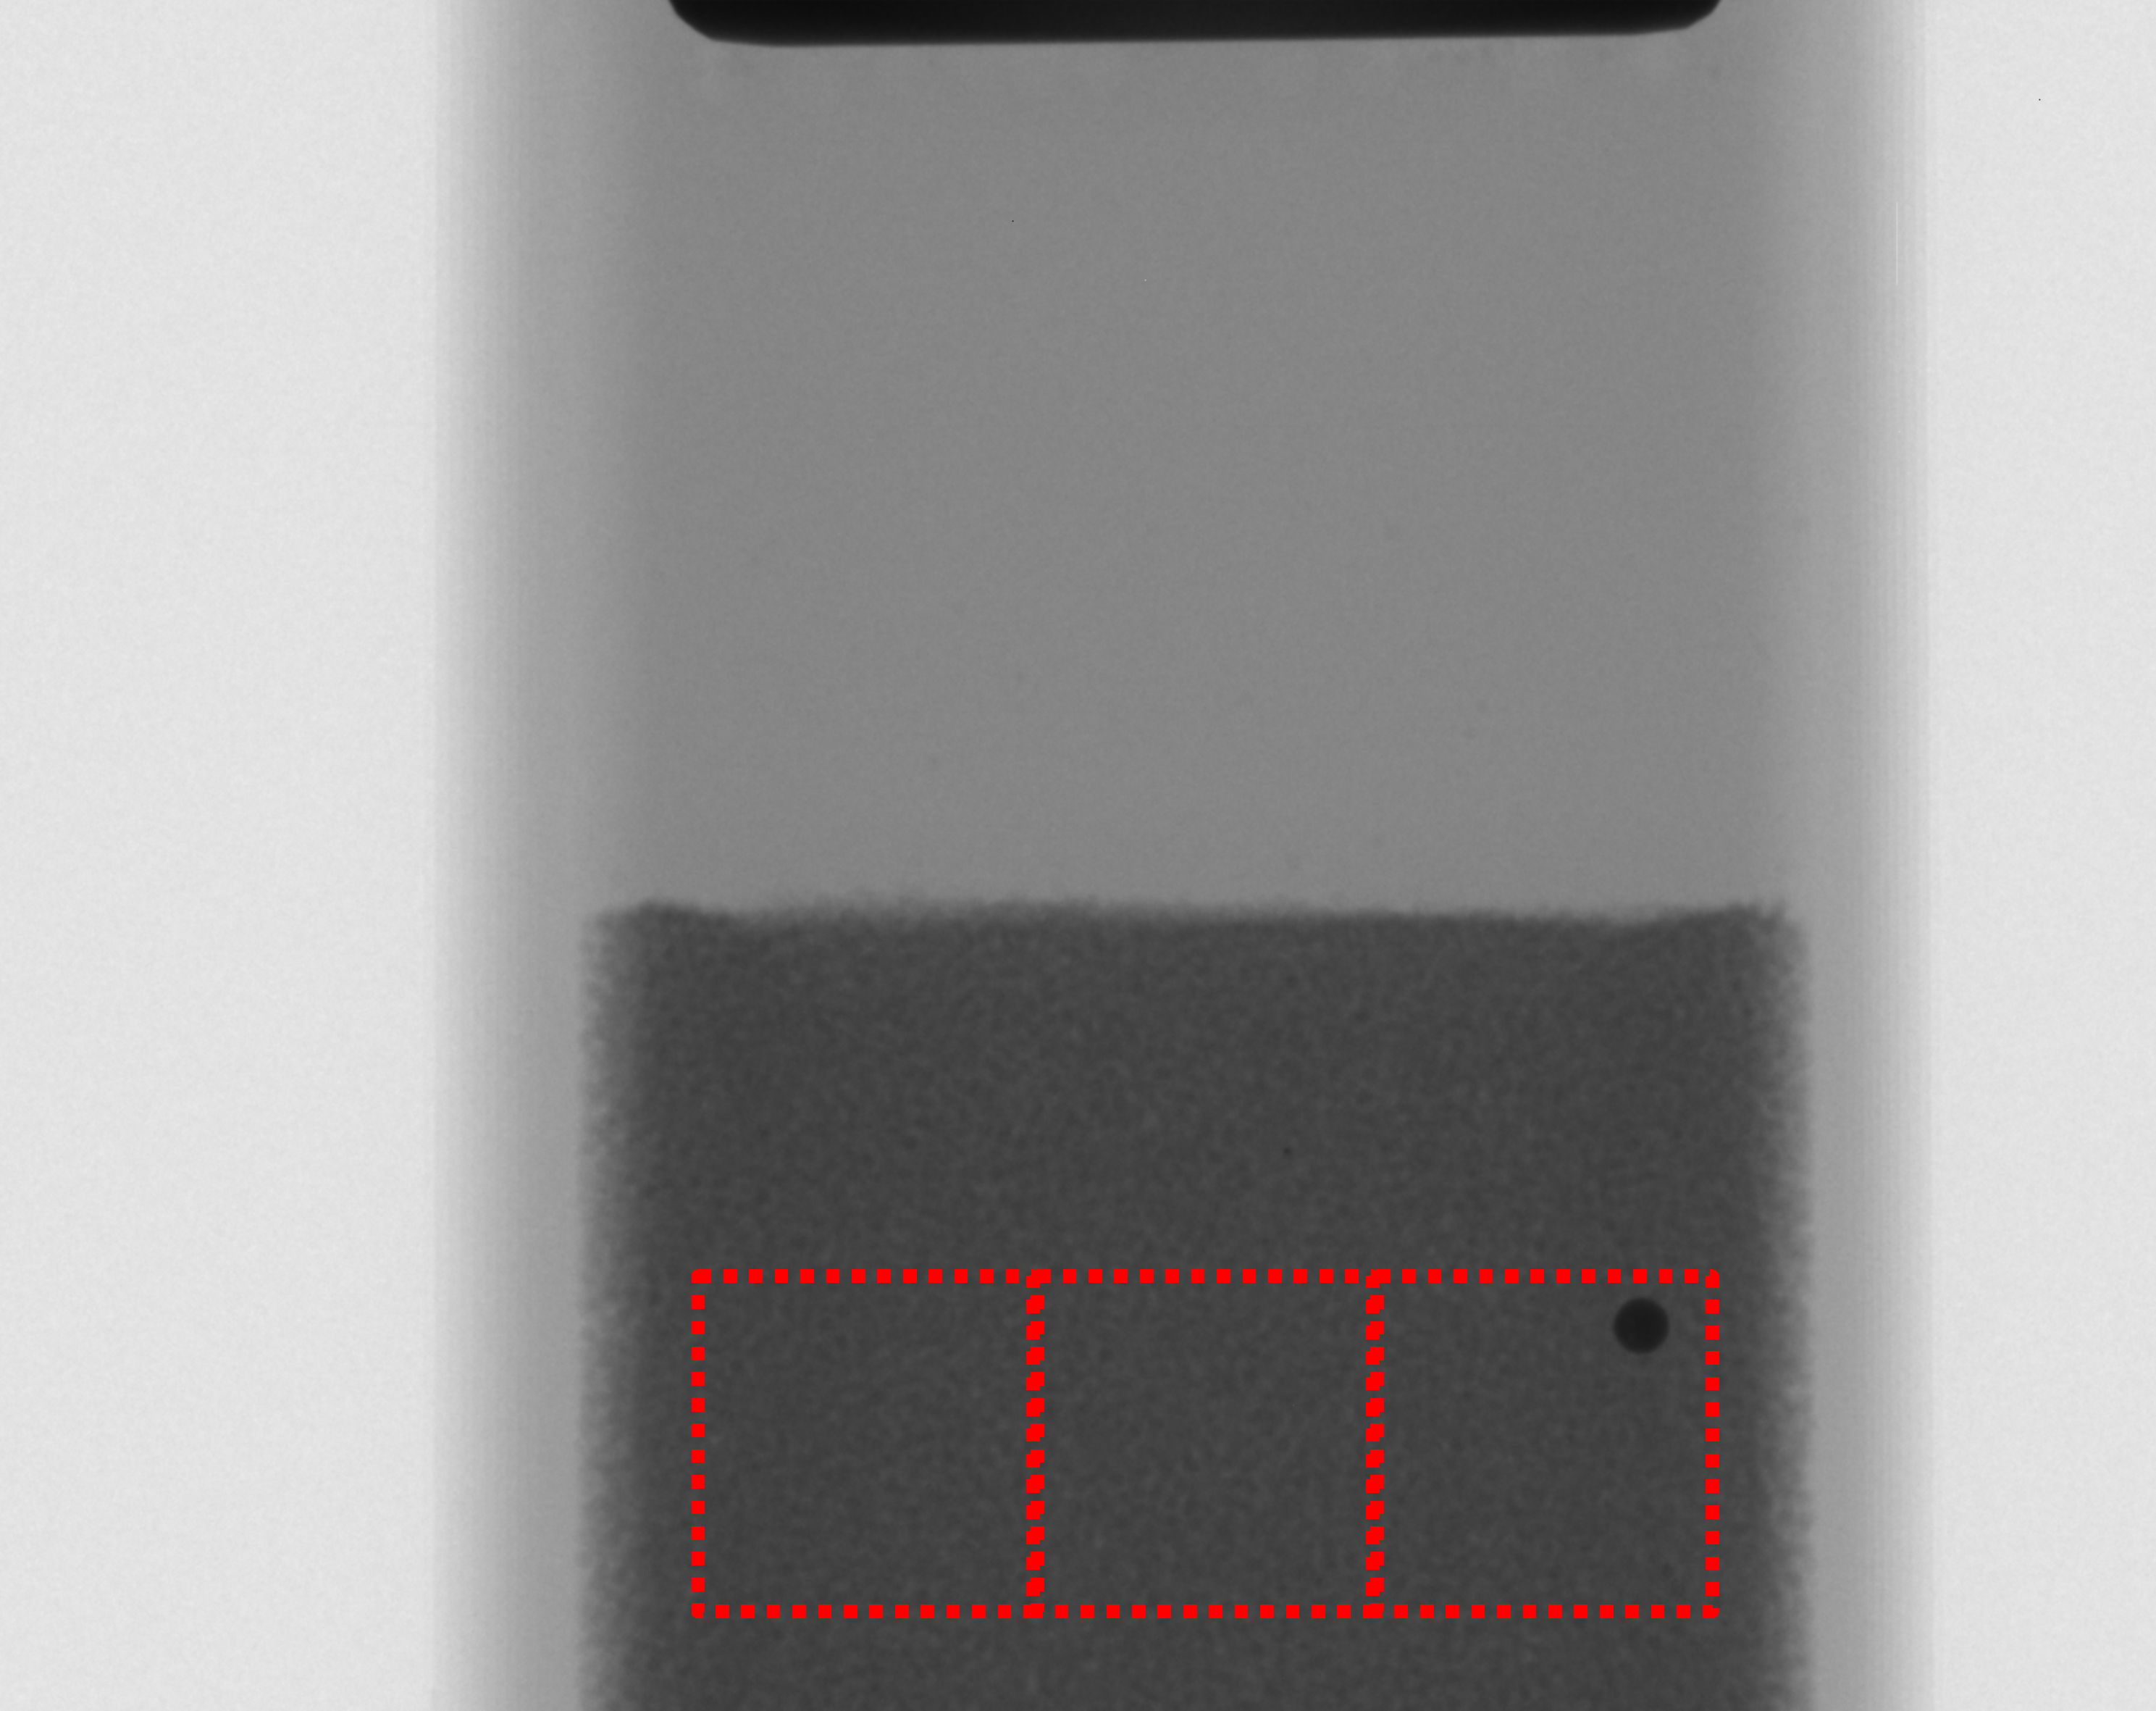
\includegraphics[width=0.9\textwidth]
	{Sources/sedimenting_bed/radiogram_rois.pdf}
\end{textblock}	


\begin{textblock}{0.45}(0.55,0.35)
\centering
\movie[width =0.6\textwidth, poster, loop]
{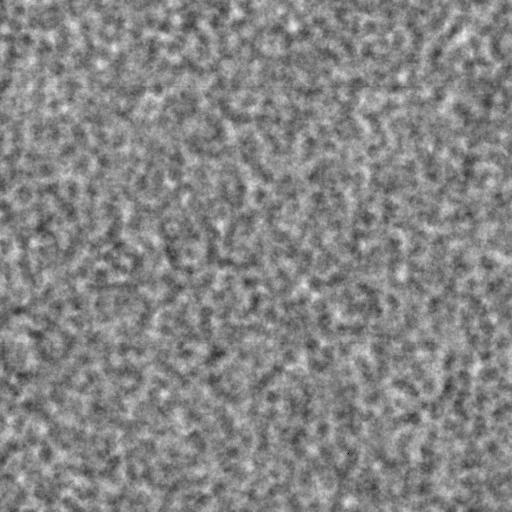
\includegraphics[width=0.6\textwidth]{Sources/sedimenting_bed/sedimentationROI.png}}
{videos/02_750ul_per_min_original.avi}
\end{textblock}

}


%%%%%%%%%%%%%%%%%%%%%%%%%%% Image structure function %%%%%%%%%%%%%%%%%%%
\frame{
\begin{tikzpicture}[remember picture,overlay]
\fill[blue1]
(current page.north west) rectangle ([xshift=0.55\paperwidth,yshift=0.33\paperheight]current page.west|-{pic cs:end});
\end{tikzpicture}

\begin{textblock}{0.8}(0.02,0.03)
	\textcolor{white}{
		\Large The image structure function $D(\mathbf{q},\tau)$}
\end{textblock}

\begin{textblock}{0.6}(0.02,0.1)
\centering
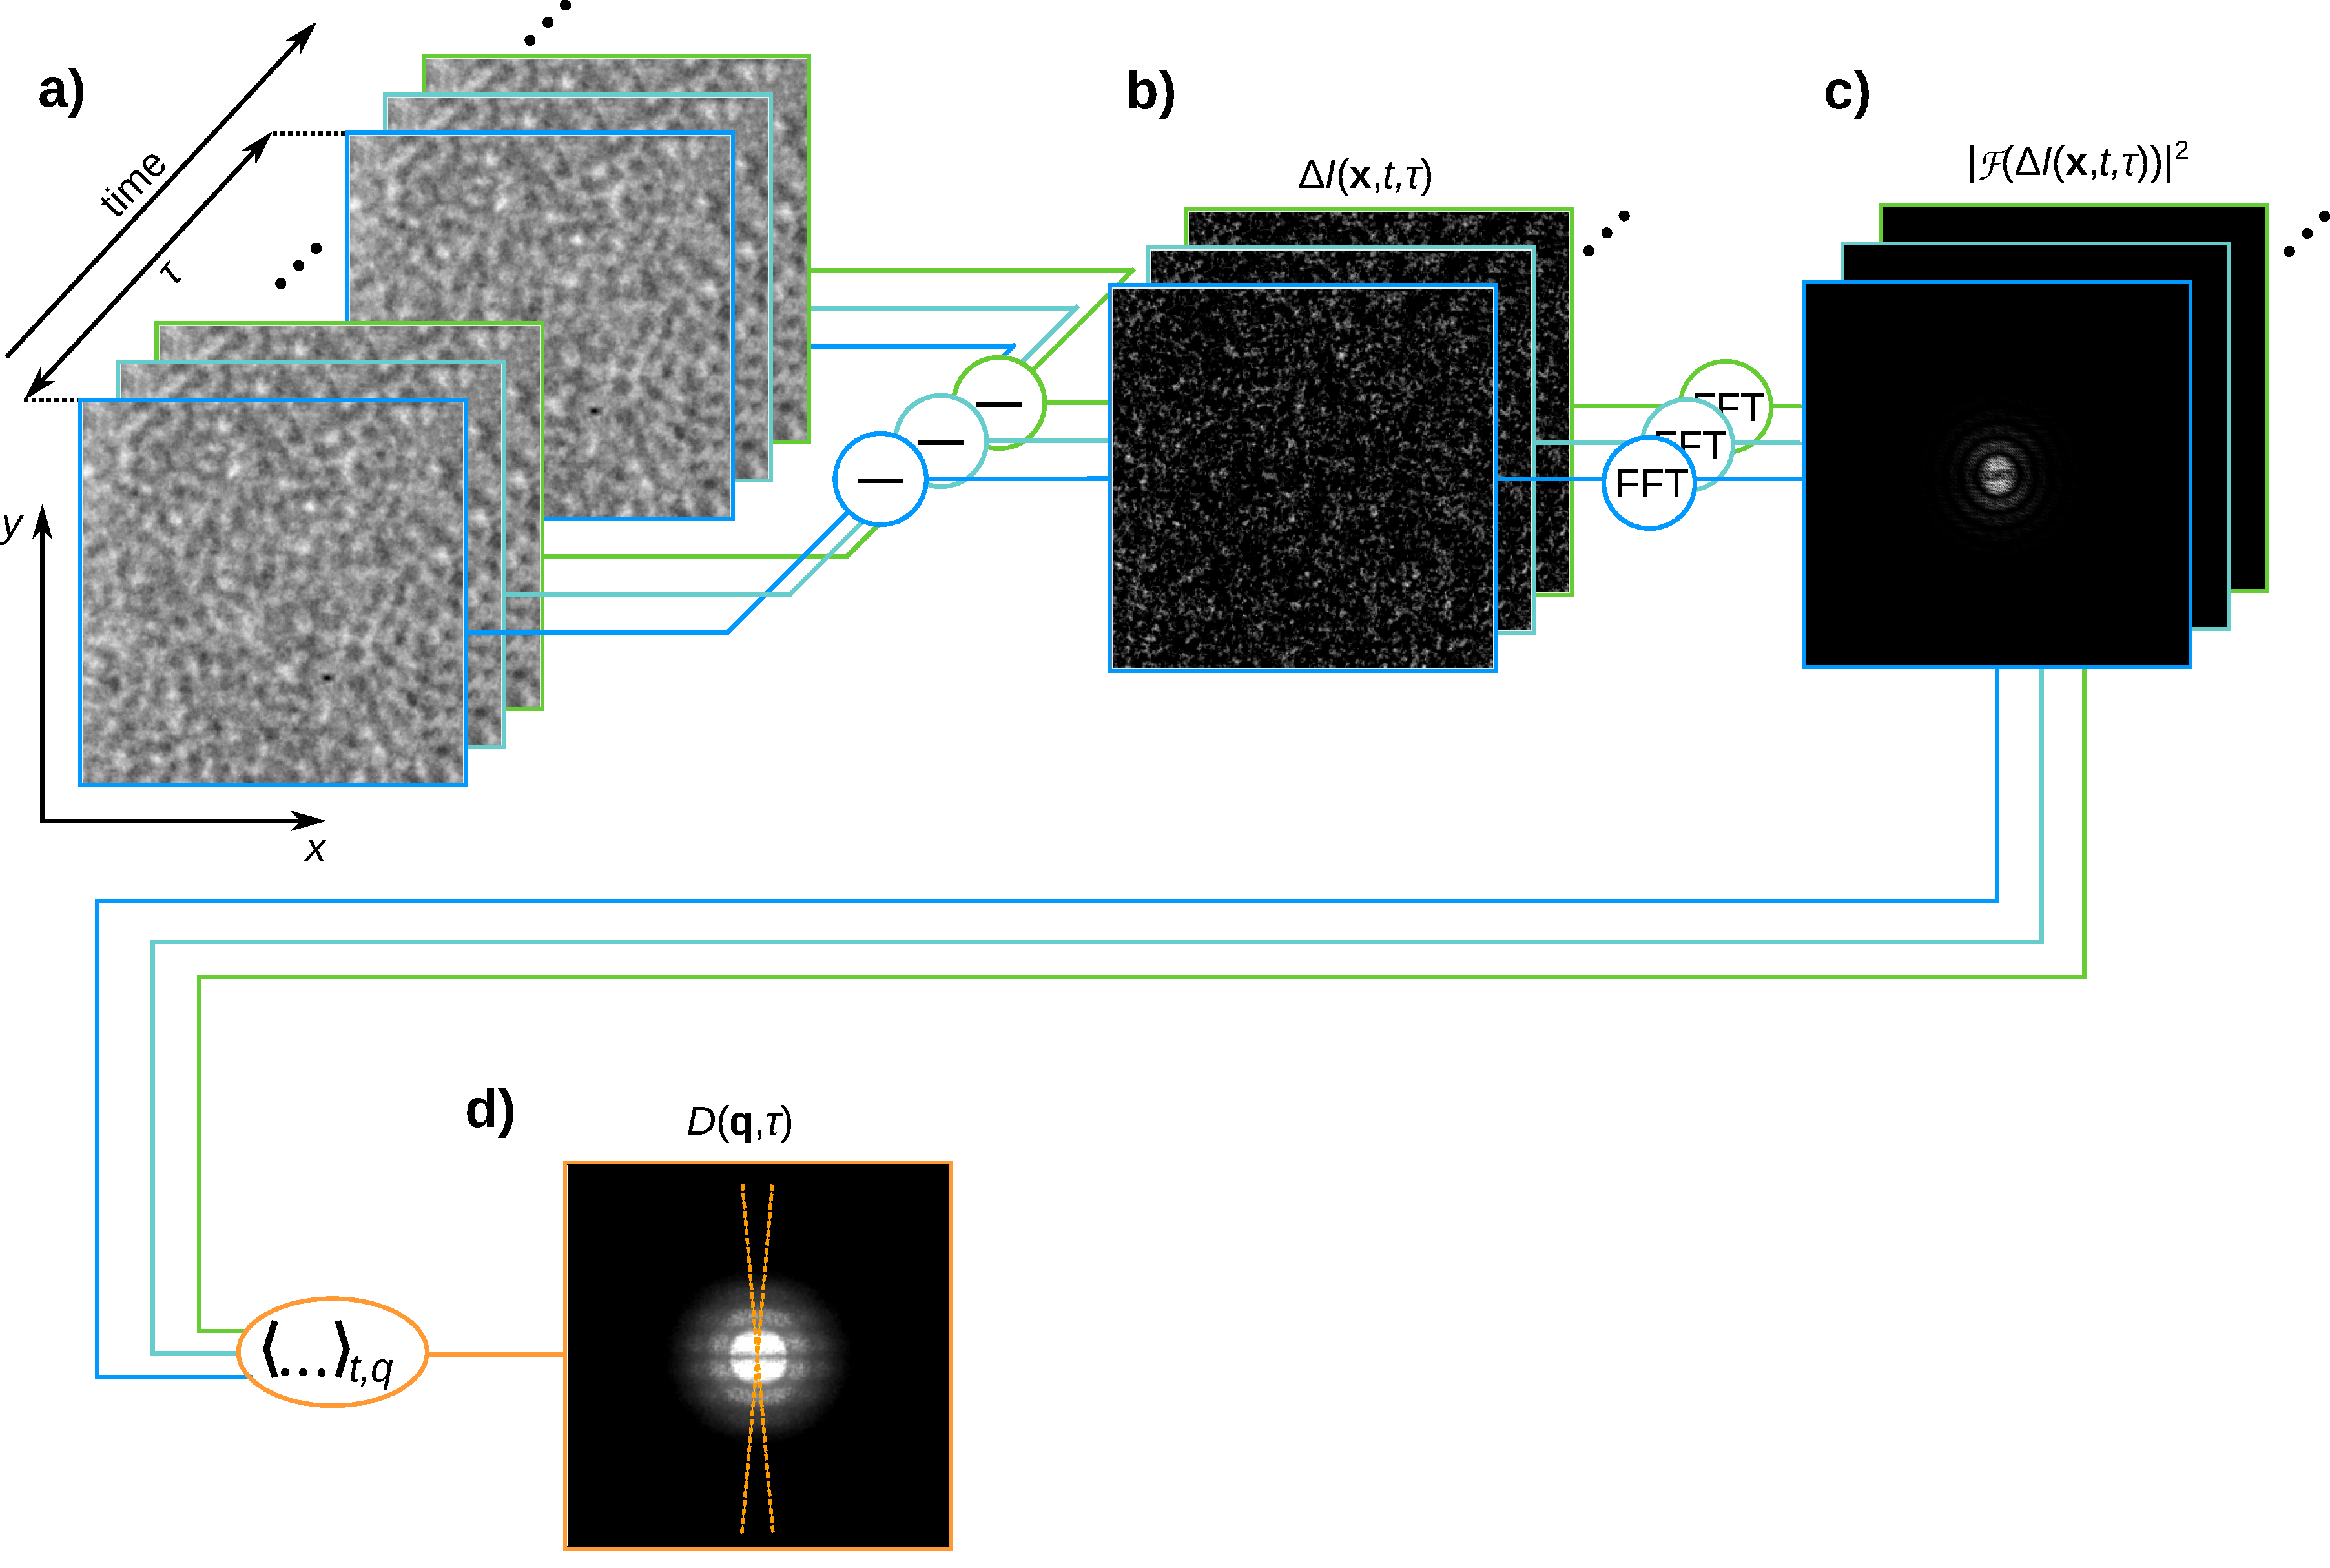
\includegraphics[width=\textwidth]{Sources/sedimenting_bed/image_structure_function.pdf}
\end{textblock}

\begin{textblock}{0.5}(0.48,0.52)
\visible<2->{
	\begin{align}
	D(\mathbf{q},\tau)
	&= \Big\langle |I(\mathbf{q}, t+\tau) - I(\mathbf{q},t)|^2  \Big\rangle_t \nonumber \\
	&= A(\mathbf{q})
	\bigg[1-
	\textcolor{red}{
		\frac{\big\langle I^*(\mathbf{q},t) I(\mathbf{q},t+\tau) \big\rangle_t}
		{\big\langle |I(\mathbf{q},t)|^2 \big\rangle_t}
	}
	\bigg] 
	+ B(\mathbf{q})\nonumber
	\end{align}
	
	\begin{itemize}
		\item $D(\mathbf{q}, \tau \rightarrow 0) = B(\mathbf{q})$
		\item $D(\mathbf{q}, \tau \rightarrow \infty) = A(\mathbf{q}) + B(\mathbf{q})$
	\end{itemize}
	}
\end{textblock}

\begin{textblock}{0.5}(0.55,0.1)
\only<3>{
	\centering
	\colorbox{lightblue}{
		Linear space invariant imaging}
	\begin{align}
	\textcolor{red}{
	f(\mathbf{q},\tau) = \frac
	{\langle \rho^*(\mathbf{q},t) \rho(\mathbf{q},t+\tau) \rangle_t}
	{\langle |\rho(\mathbf{\mathbf{q}},t)|^2 \rangle_t}}
	\nonumber
	\end{align}
	\textcolor{red}{
	Intermediate scattering function}}
\end{textblock}


\begin{textblock}{0.9}(0.02,0.95)
	{\scriptsize
	In collaboration with Manuel Escobedo, University of Düsseldorf}
\end{textblock}
}



%%%%%%%%%%% linear space invariant imaging %%%%%%%%%%%%%%
\frame{
\begin{tikzpicture}[remember picture,overlay]
\fill[blue1]
(current page.north west) rectangle ([xshift=0.58\paperwidth,yshift=0.33\paperheight]current page.west|-{pic cs:end});
\end{tikzpicture}

\begin{textblock}{0.8}(0.02,0.03)
	\textcolor{white}{
		\Large X-ray imaging -- Linear space invariant?}
\end{textblock}

\begin{textblock}{0.4}(0.05,0.12)	
	\centering
	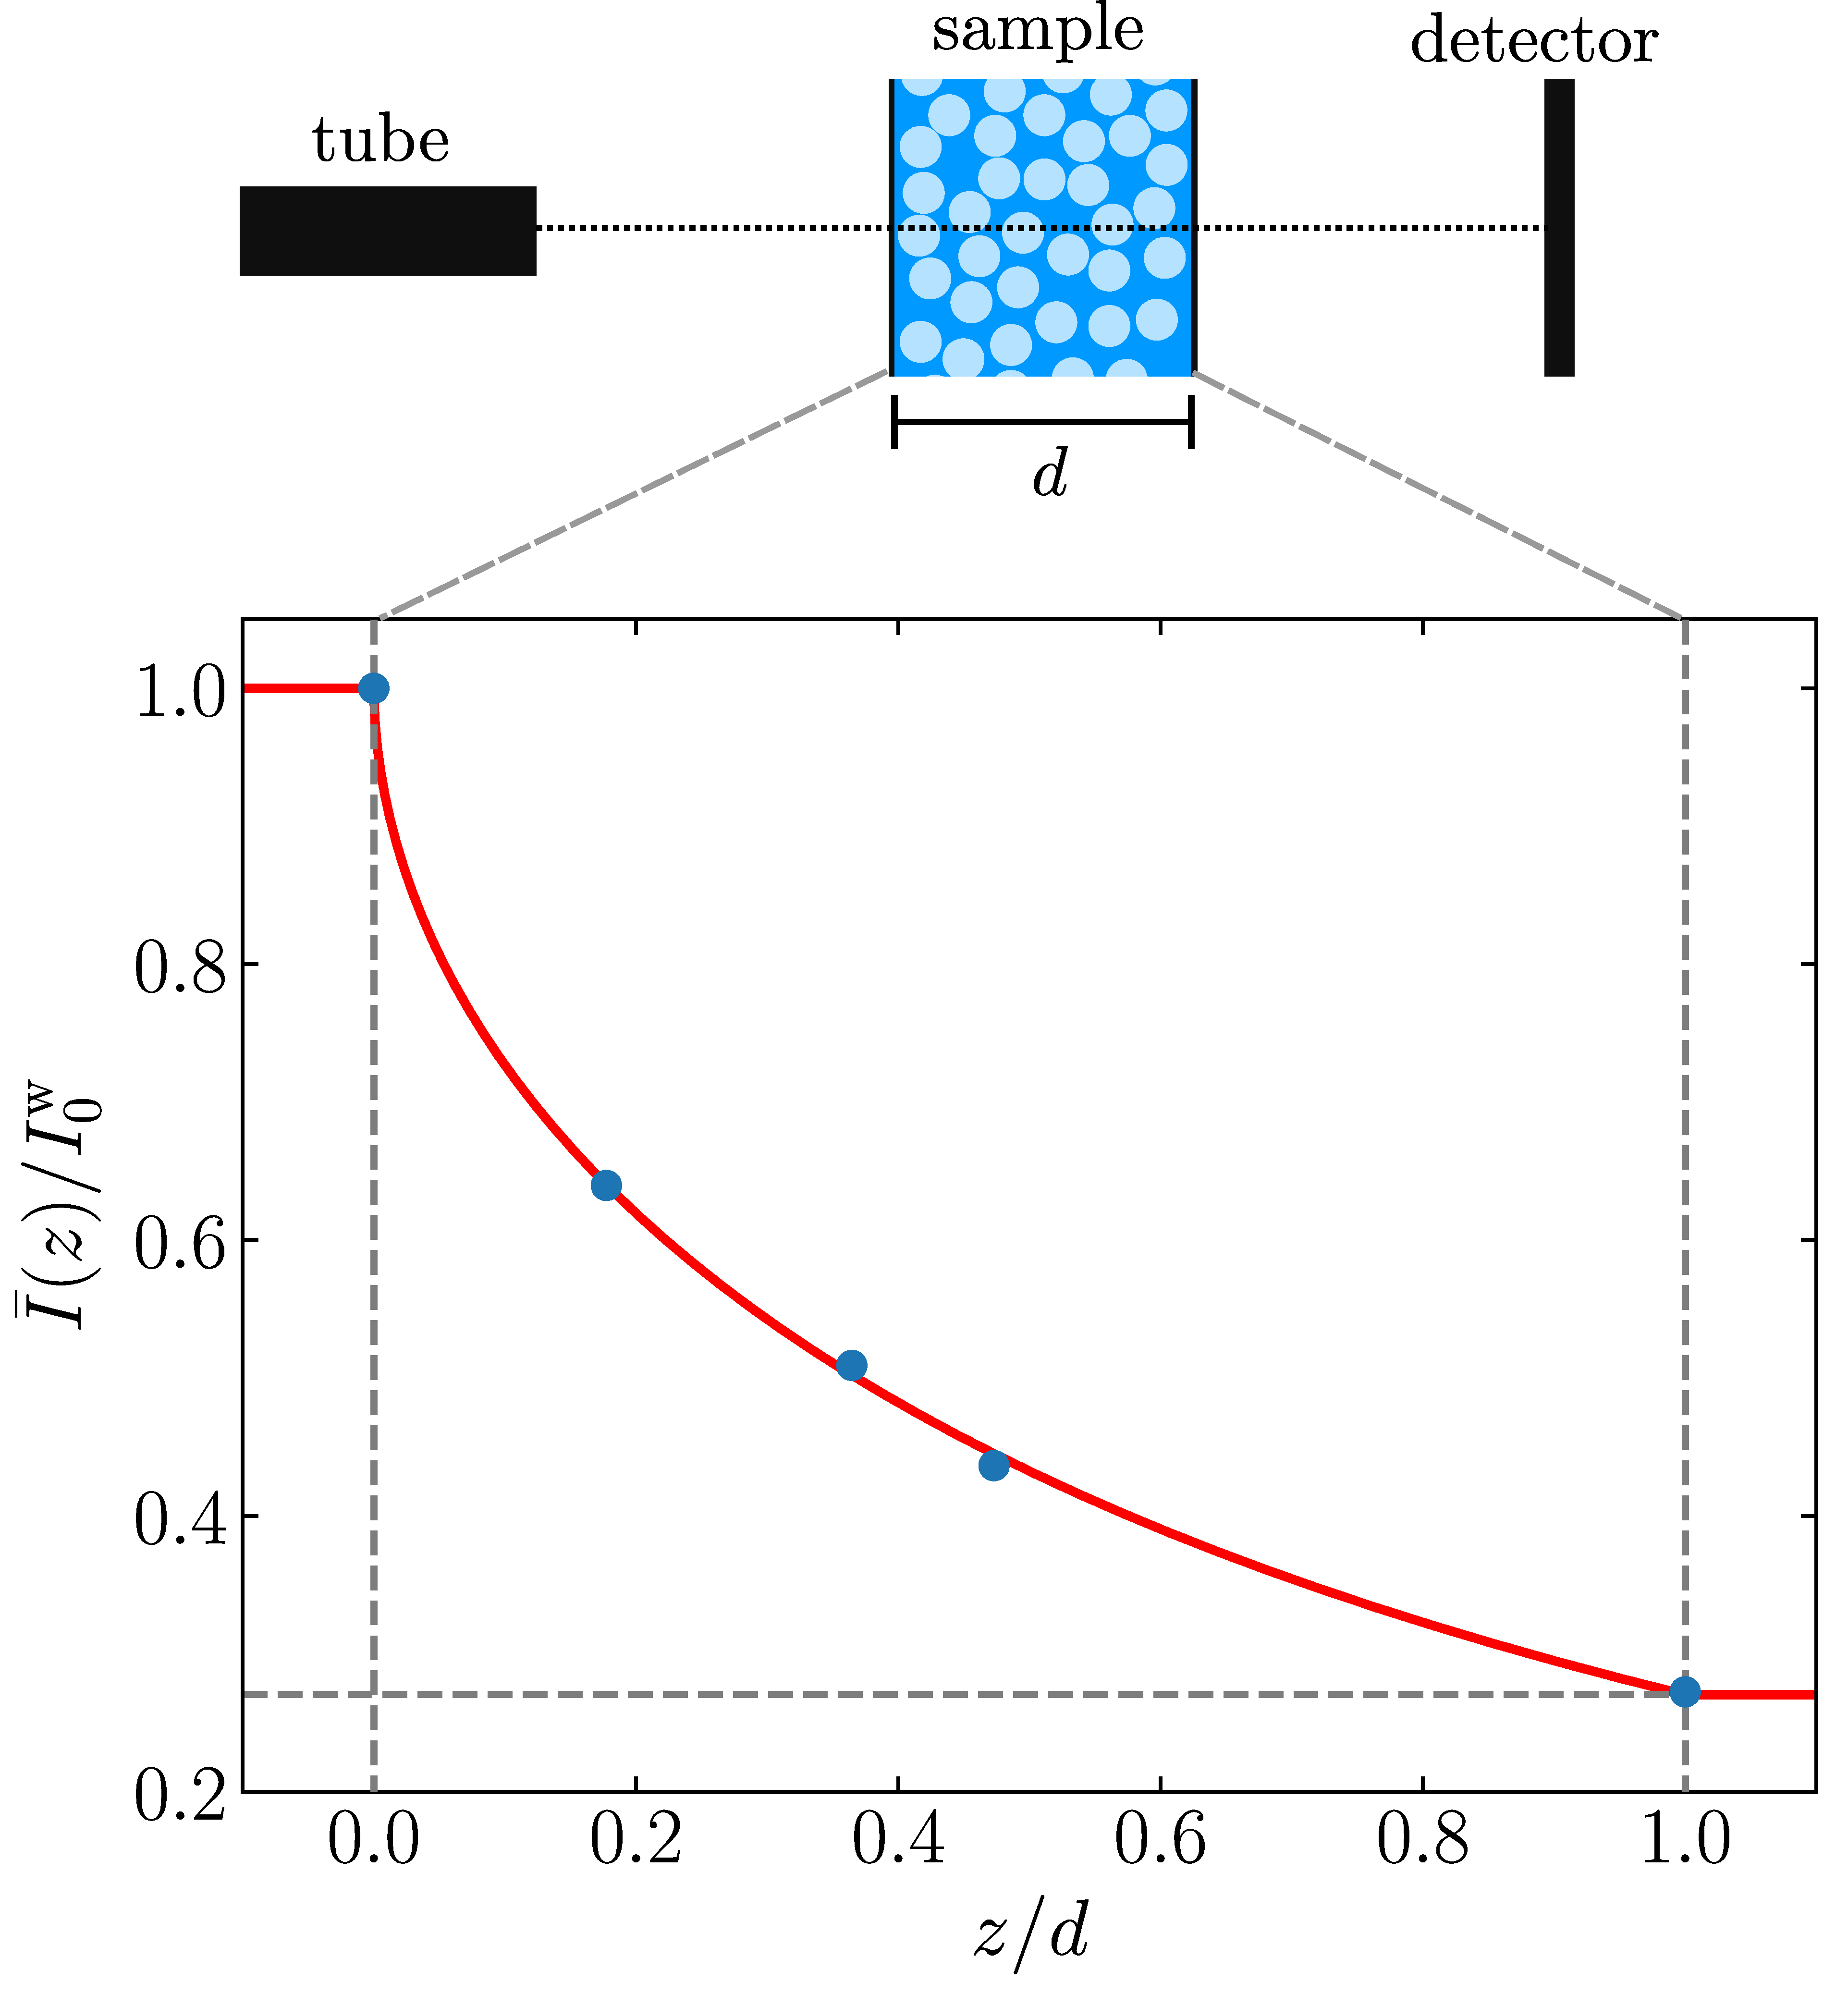
\includegraphics[width=\textwidth]{Sources/sedimenting_bed/I_over_I0_vs_z.pdf}
\end{textblock}

\begin{textblock}{0.35}(0.2,0.4)	
	\centering
	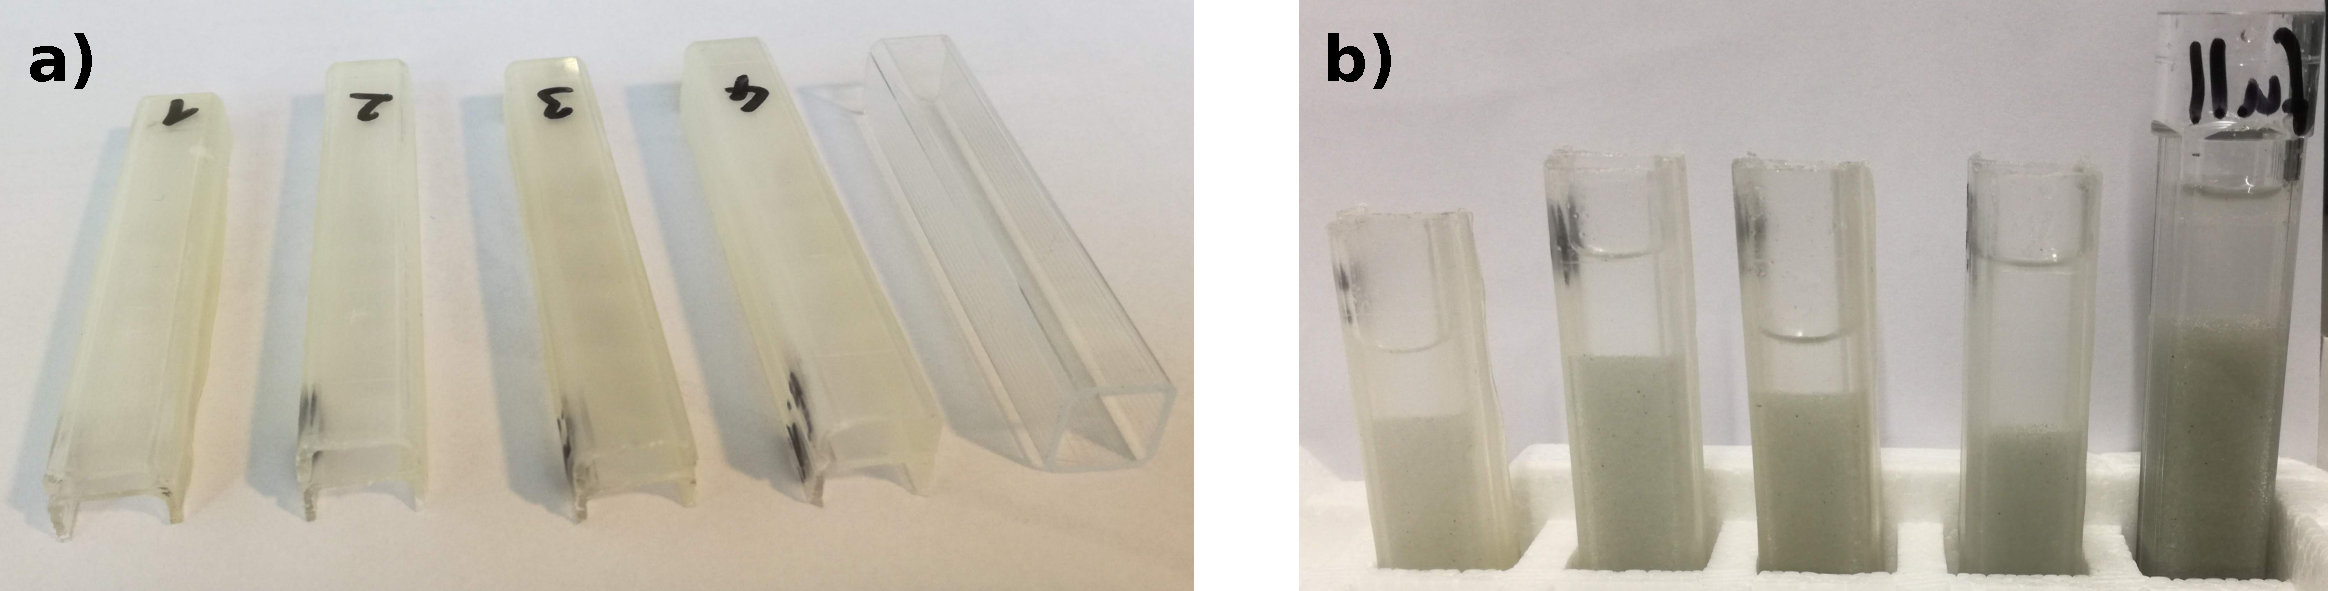
\includegraphics[width=\textwidth]{Sources/sedimenting_bed/cuvettes_beam_hardening.pdf}
\end{textblock}

\begin{textblock}{0.4}(0.05,0.12)	
\centering
\visible<2->{
\includegraphics[width=\textwidth]{Sources/sedimenting_bed/cross.pdf}}
\end{textblock}

\begin{textblock}{0.4}(0.59,0.05)	
\centering
\visible<3->{
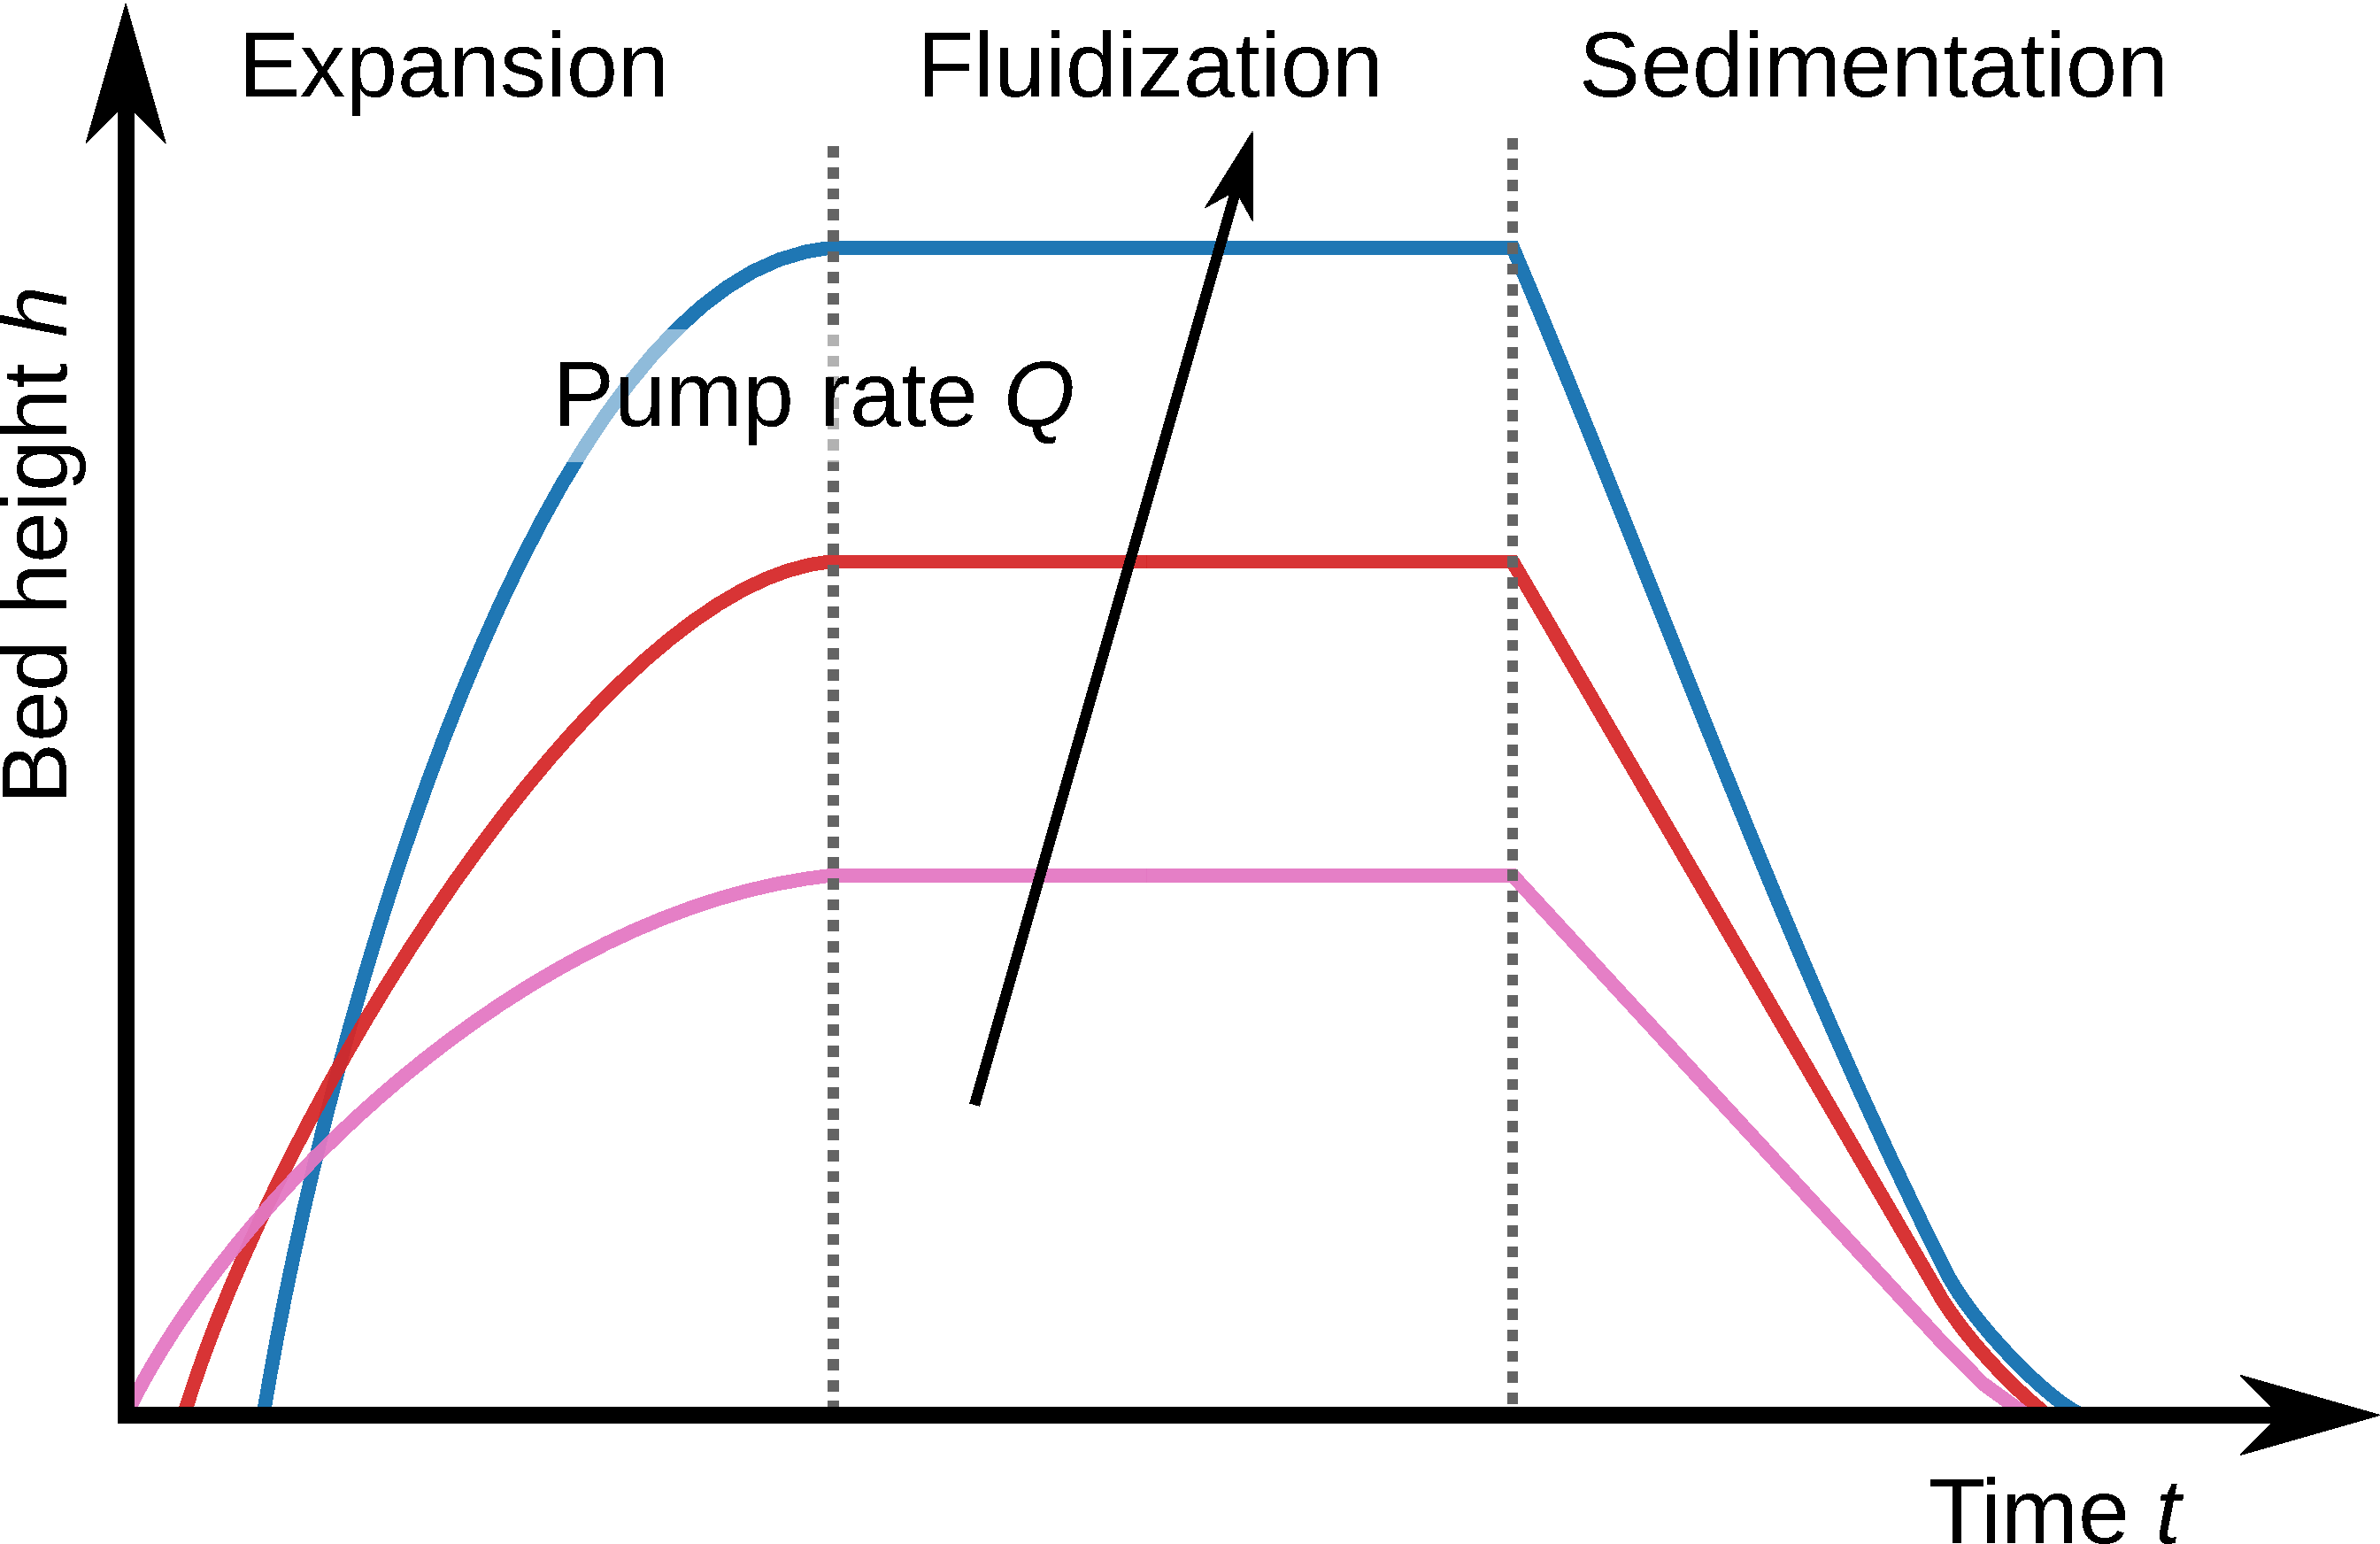
\includegraphics[width=0.8\textwidth]{Sources/sedimenting_bed/setup-fluidized_bed_right.pdf}}
\end{textblock}

\begin{textblock}{0.38}(0.59,0.45)
	\visible<3->{
	\centering
	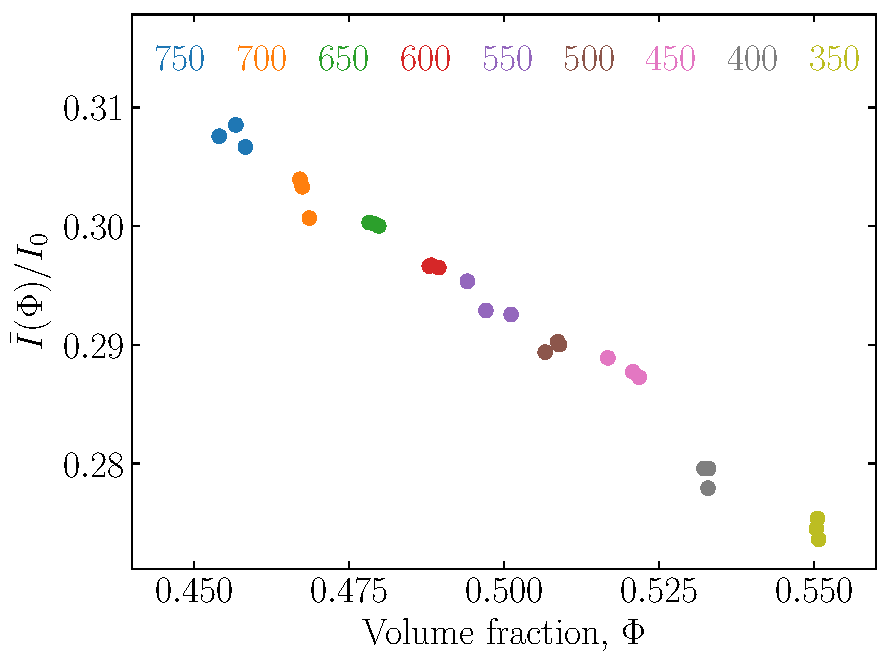
\includegraphics[width=\textwidth]
	{Sources/sedimenting_bed/I_over_I0_vs_Phi.pdf}}
\end{textblock}

\begin{textblock}{0.35}(0.67,0.8)	
	\visible<3->{
		\colorbox{lightblue}{
		$0.45 <  \Phi < 0.56$}}
\end{textblock}

\begin{textblock}{0.35}(0.85,0.6)	
	\visible<3->{
		\fbox{
		\textcolor{darkgreen}{\Huge $\checkmark$}}}
\end{textblock}
}


\frame{
\begin{tikzpicture}[remember picture,overlay]
\fill[blue1]
(current page.north west) rectangle ([xshift=0.69\paperwidth,yshift=0.33\paperheight]current page.west|-{pic cs:end});
\end{tikzpicture}

\begin{textblock}{0.8}(0.02,0.03)
	\textcolor{white}{
		\Large X-DFA for a suspension of sedimenting particles}
\end{textblock}	


\begin{textblock}{0.9}(0.05,0.05)
	\begin{align}
	f(q,\tau) = 
	\cos(q \langle v_\text{s} \rangle \tau)
	\exp\left(- \frac{1}{2} q^2 \delta v^2 \tau^2 \right)
	\nonumber
	\end{align}
	\centering
	$\langle v_\text{s} \rangle = \langle \Delta r \rangle / \tau_\nu, 
	\langle \delta v \rangle = \langle \delta r \rangle / \tau_{\delta \nu}$
\end{textblock}

\begin{textblock}{0.45}(0.025,0.4)	
	\centering
	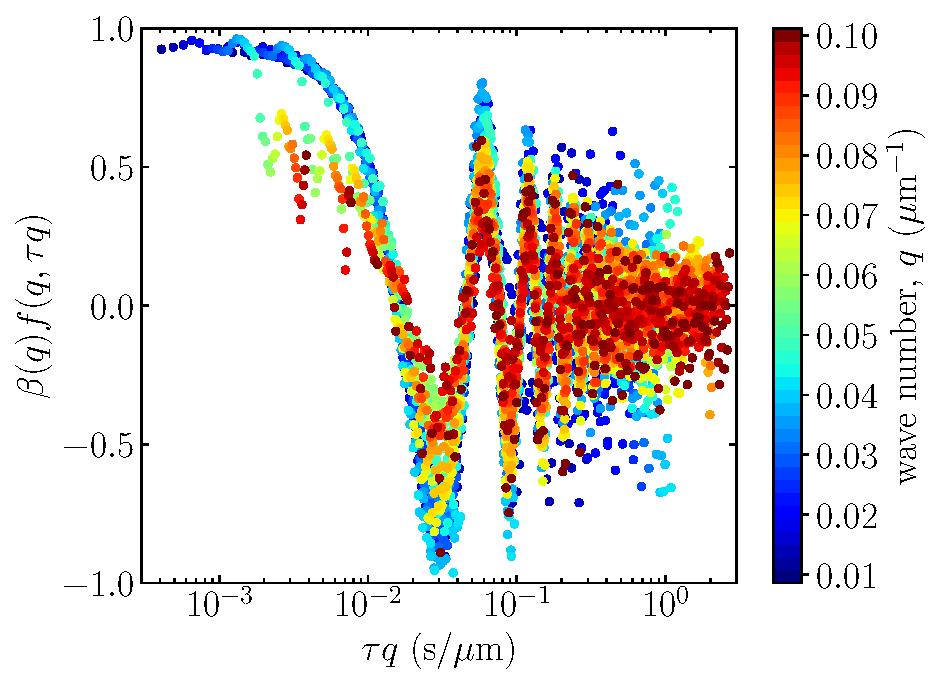
\includegraphics[width=\textwidth]
	{Sources/sedimenting_bed/fqt_tq.pdf}
\end{textblock}

\begin{textblock}{0.45}(0.5,0.4)	
	\centering
	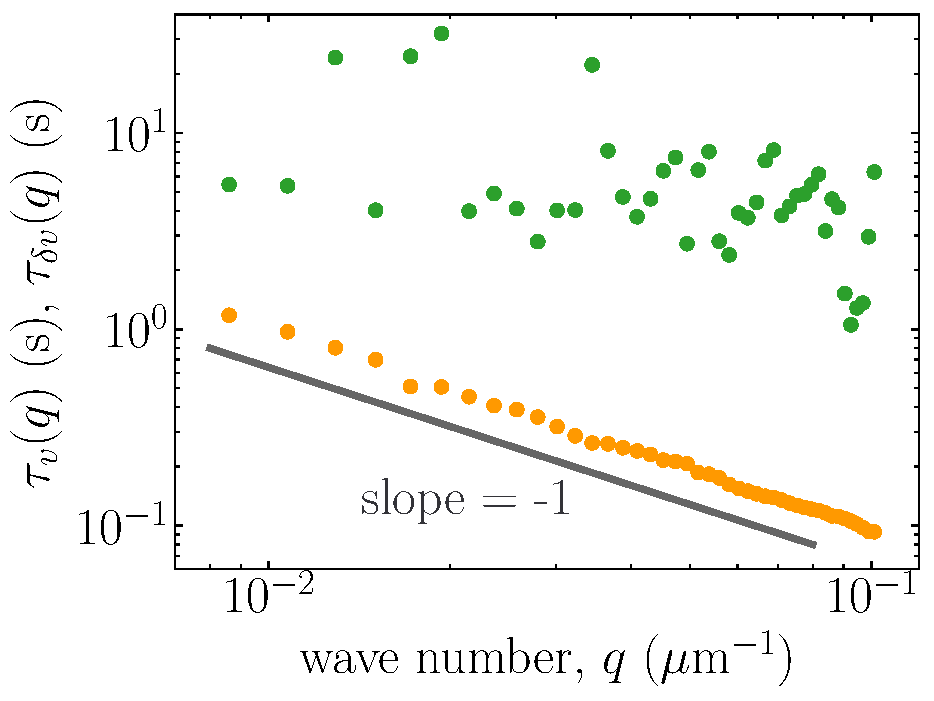
\includegraphics[width=\textwidth]
	{Sources/sedimenting_bed/tau_vs_q.pdf}
\end{textblock}
}





%%%%%%%%%%% Front tracking vs X-DFA %%%%%%%%%%%%%%%%%%%%%
\frame{
\begin{tikzpicture}[remember picture,overlay]
\fill[blue1]
(current page.north west) rectangle ([xshift=0.38\paperwidth,yshift=0.33\paperheight]current page.west|-{pic cs:end});
\end{tikzpicture}

\begin{textblock}{0.8}(0.02,0.03)
	\textcolor{white}{
		\Large Front tracking vs.\ X-DFA}
\end{textblock}

\begin{textblock}{0.45}(0.02,0.1)	
\centering
\visible<1->{
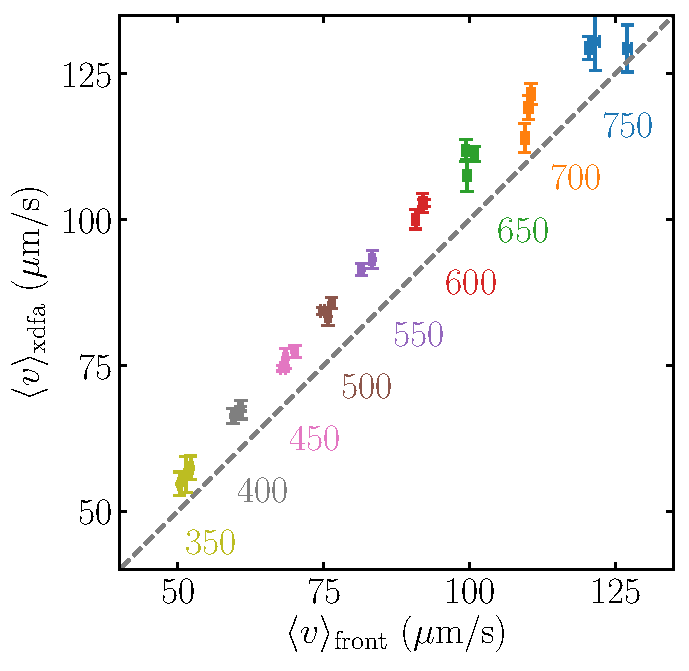
\includegraphics[width=\textwidth]
{Sources/sedimenting_bed/Sedimentation_velocites_v_front_vs_v_X-DFA.pdf}
}
\vspace{-0.3cm}
$\langle v\rangle_\text{xdfa} > \langle v \rangle_\text{front}$ by 9.4\%
\end{textblock}

\begin{textblock}{0.5}(0.5,0.15)
\centering
\visible<2->{
\movie[width =0.8\textwidth, poster, loop]	
{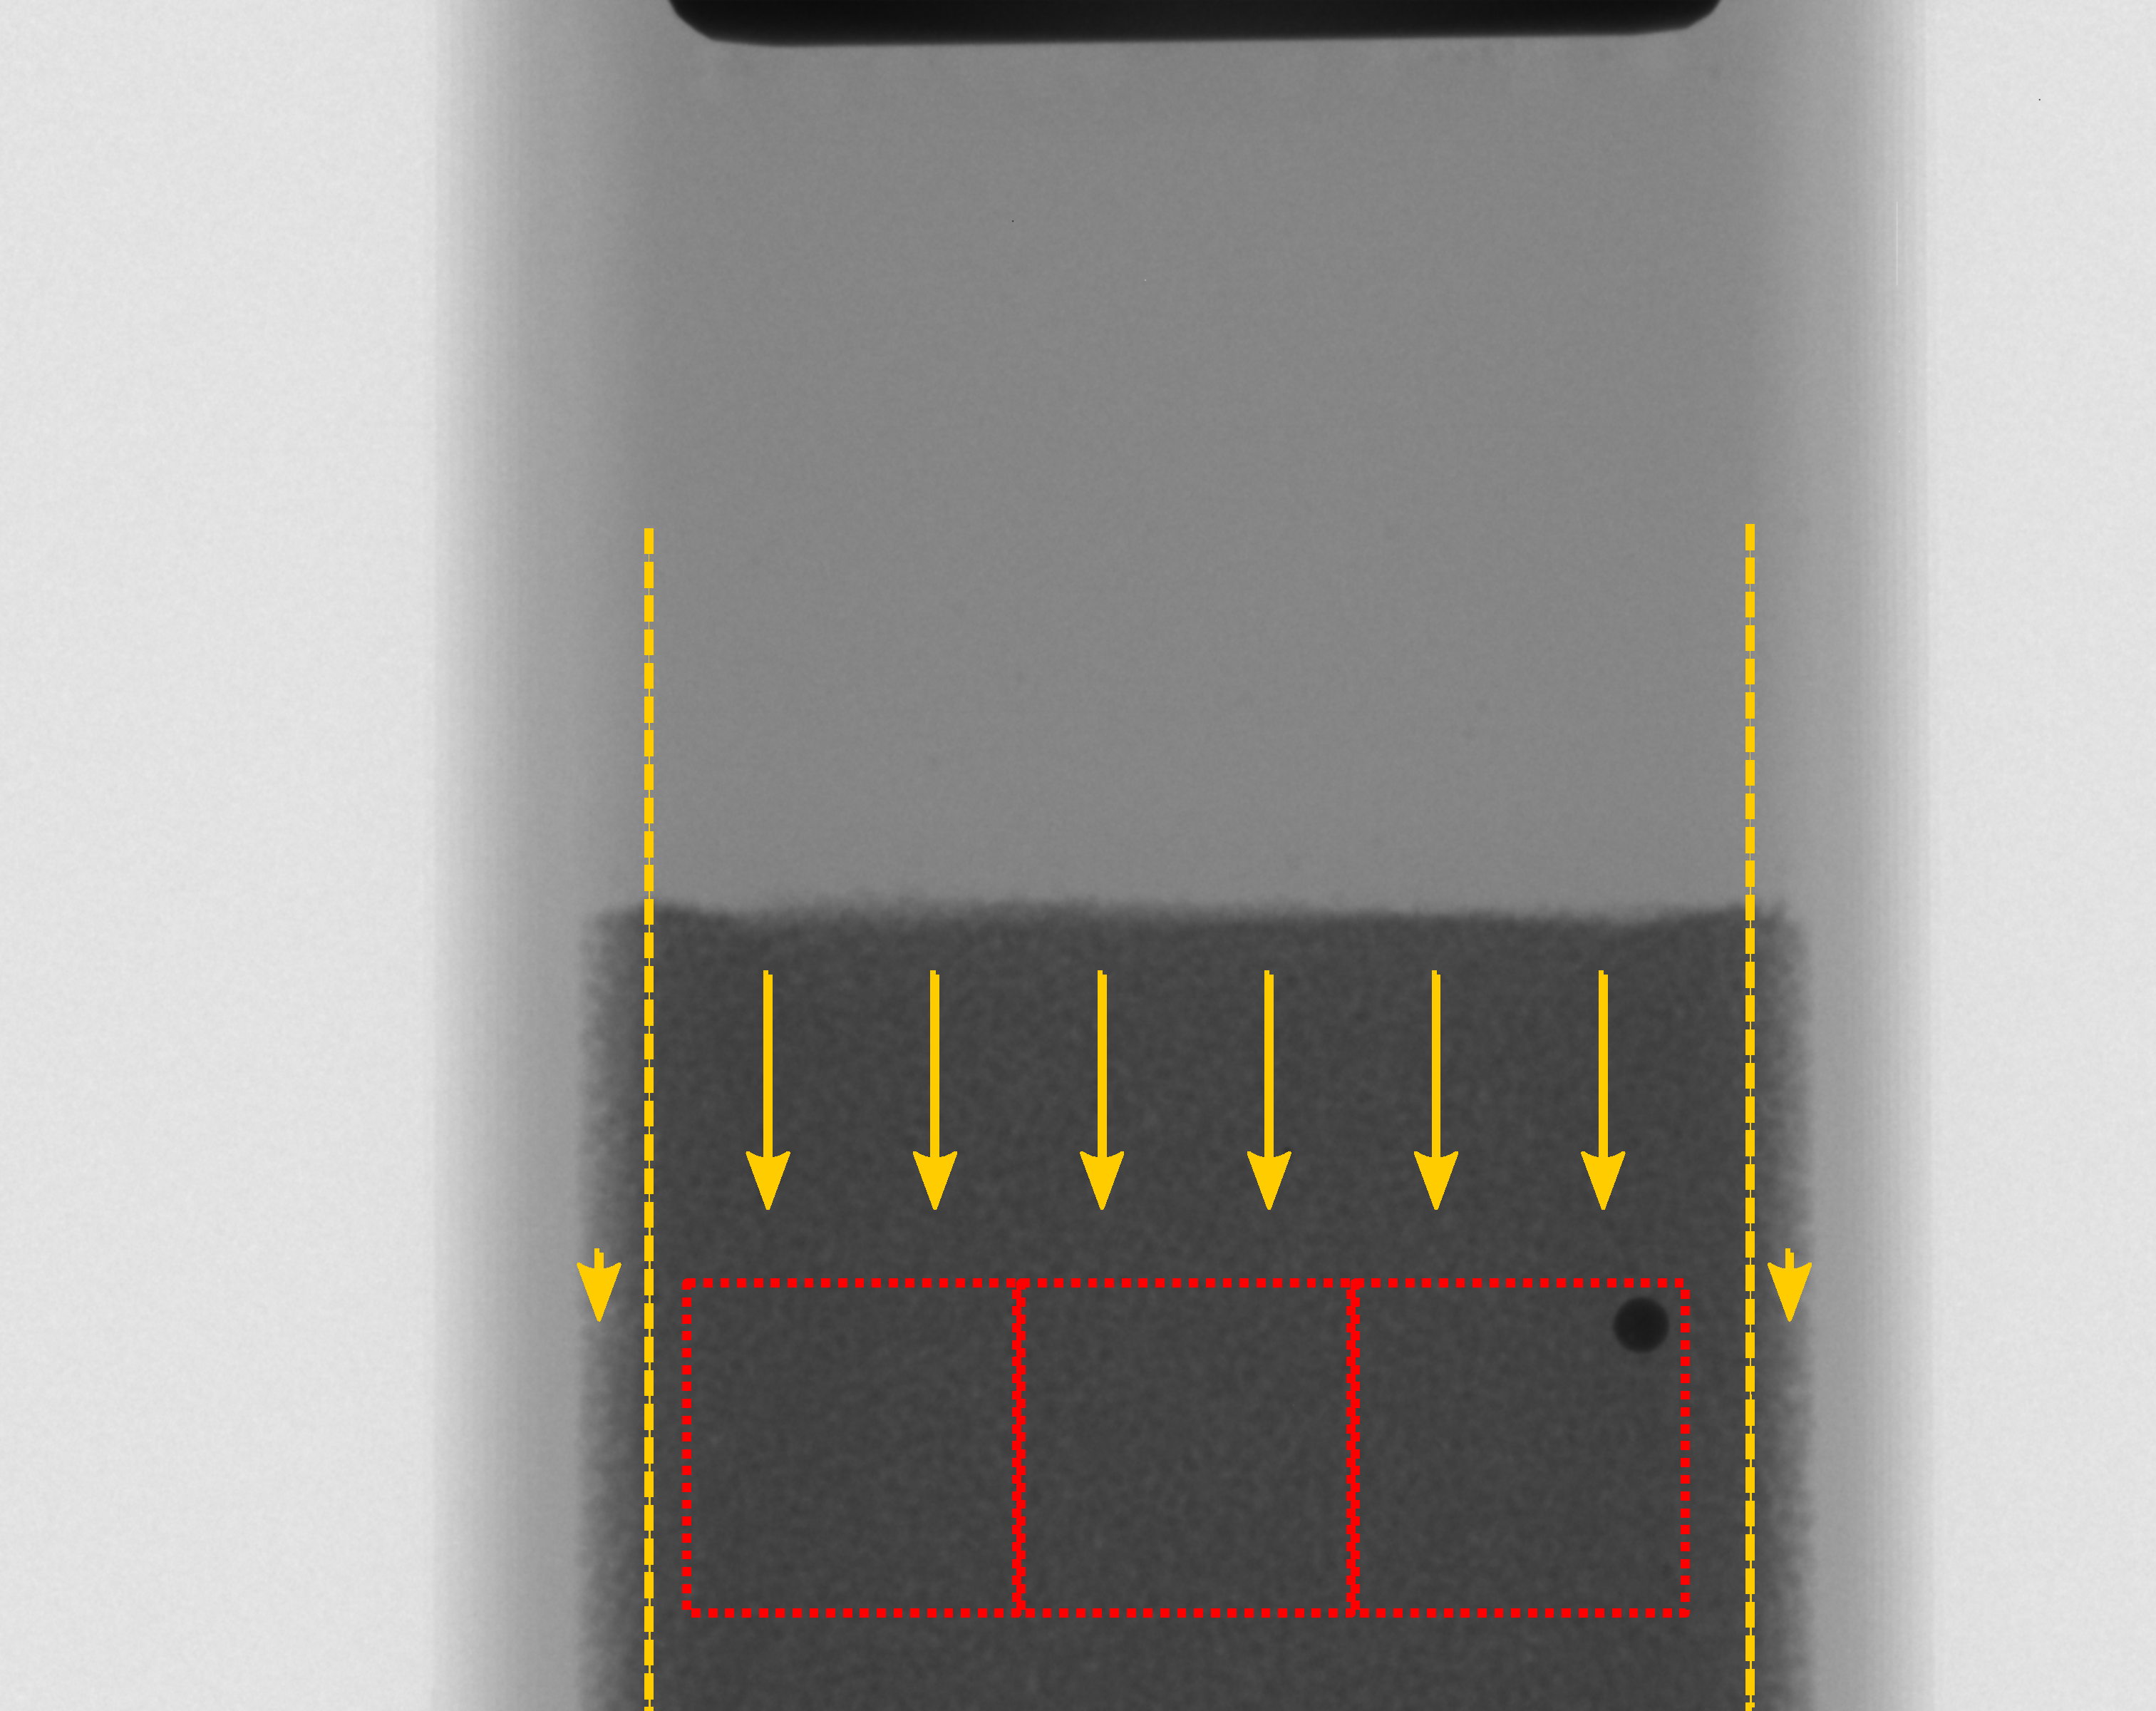
\includegraphics[width=0.8\textwidth]
{Sources/sedimenting_bed/creeping_boundary_flow.pdf}}
{videos/boundary_layer.avi}}
\end{textblock}
}

\frame{
\frametitle{Estimate width of boundary layer}
\begin{textblock}{0.45}(0.02,0.1)	
	\centering
	\visible<1->{
		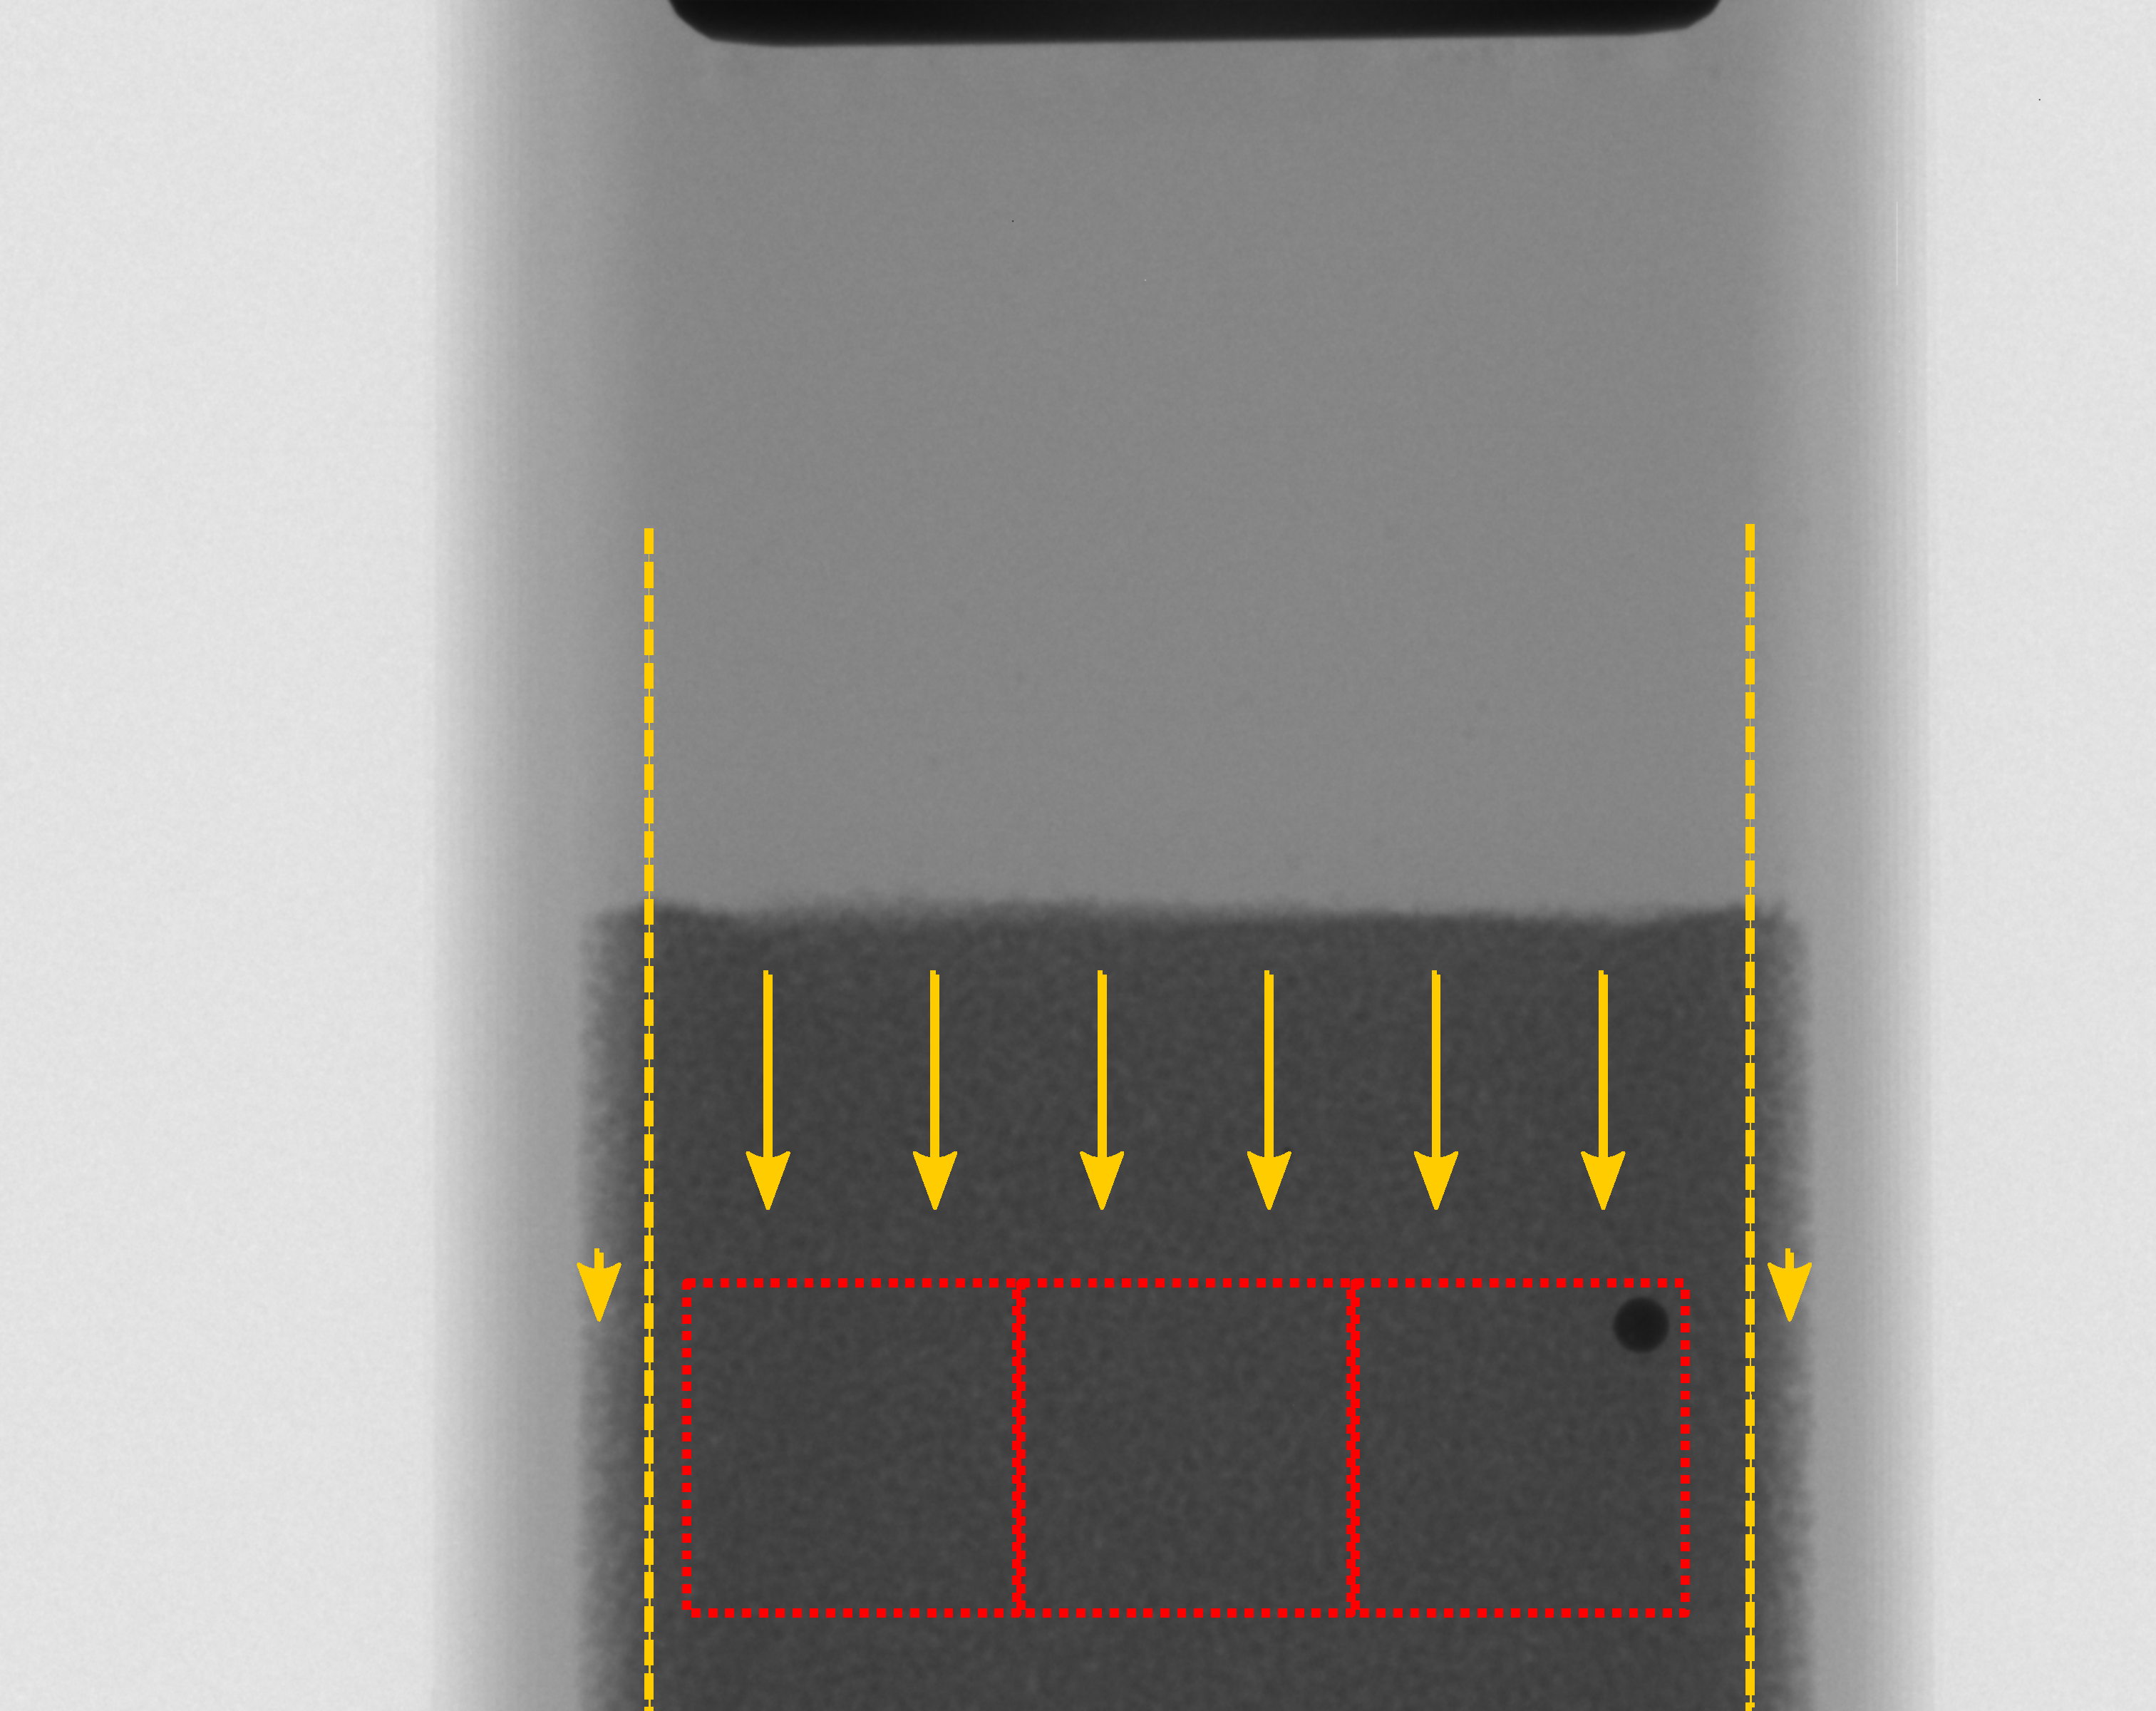
\includegraphics[width=\textwidth]
		{Sources/sedimenting_bed/creeping_boundary_flow.pdf}
	}
	$\langle v\rangle_\text{xdfa} > \langle v \rangle_\text{front}$ by 9.4\%
\end{textblock}

\begin{textblock}{0.5}(0.5,0.1)
	$\langle v\rangle_\text{xdfa}$ takes \textcolor{red}{two} layers into account\\
	$\langle v \rangle_\text{front}$ takes \textcolor{royalblue}{four} layers into account\\[0.3cm]
	
	
\includegraphics[width=0.9\textwidth]
	{Sources/sedimenting_bed/sketch_boundary_flow.pdf}\\[0.3cm]
%	\vspace{0.6cm}
	\textbf{Estimation:}\\
	Boundary velocity = 0\\
	Else = const.\\
	$\rightarrow b \approx 3$ particle diameters
\end{textblock}

}

\frame{
\begin{textblock}{1.}(0.0,0.0)
	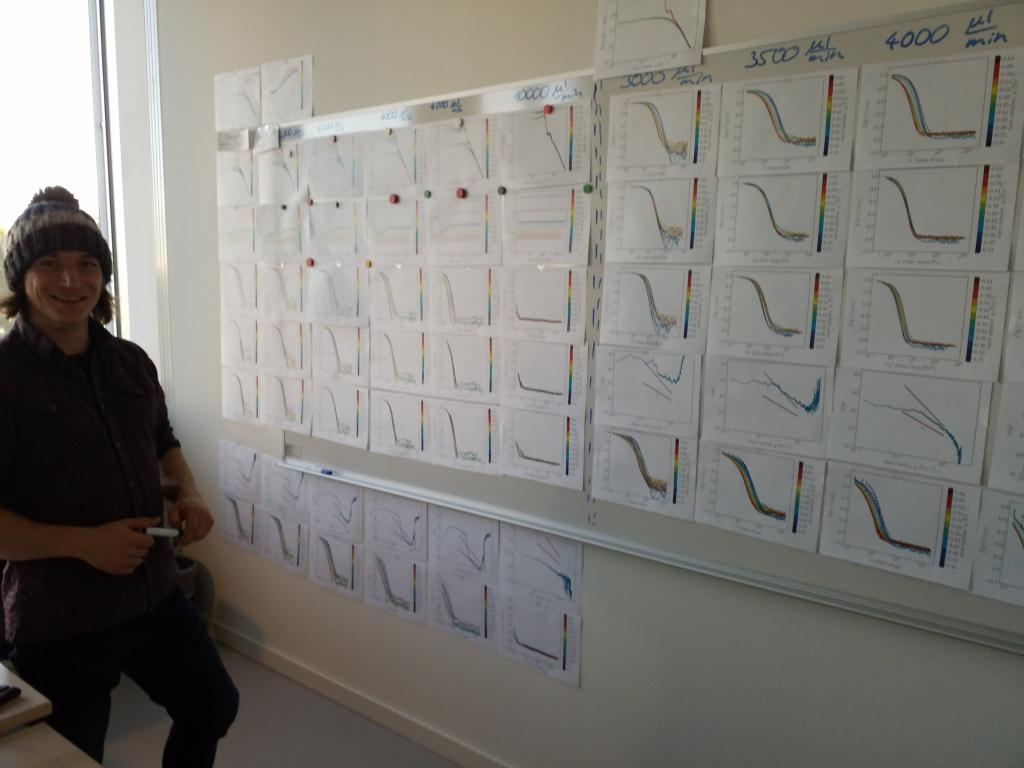
\includegraphics[width=\textwidth]
	{Sources/sedimenting_bed/whiteboard.jpg}
\end{textblock}

\begin{textblock}{0.8}(0.2,0.3)
	\colorbox{blue1}{\Huge \textcolor{white}{Thank you for your attention!}}
\end{textblock}
}



